\chapter[Evaluating Obfuscation Resilience]{Evaluating Obfuscation Resilience for Programming Assignments}\label{cha:code-eval}

In this chapter, we evaluate our defense mechanisms against automated obfuscation attacks (\contribution{3}) with datasets from real-world programming assignments. Thus, this chapter addresses our first evaluation goal (\gref{1}).
This evaluation stage thus shows that our defense mechanisms provide obfuscation resilience against all categories of the obfuscation attack classification discussed in our threat model (see \autoref{sec:threatmodel-categorization}). Note that this stage only includes the defense mechanisms that apply to programming languages, namely token sequence normalization, subsequence match merging, and the combination of both. The evaluation for modeling languages follows in the second evaluation stage.
In this evaluation stage, we use JPlag as a baseline, as it is state-of-the-art for programming assignments.
%
The evaluation is based on six real-world datasets, totaling 758 original and 968 automatically obfuscated programs.
In sum, these programs consist of over 14,000 files and close to one million lines of code.
%This yields a total of 289,046 pairwise comparisons.
We provide a replication package~\fancycite{replication-package}.

Our results demonstrate that our defense mechanisms offer broad obfuscation resilience across diverse datasets and attack types, thus significantly advancing resilience against automated obfuscation attacks.
%
Notably, we achieved a median similarity difference increase of up to 99.65 percentage points against semantic-preserving insertion-based obfuscation. We also show substantial improvements against alteration-based attacks (up to 42 percentage points) and refactoring-based attacks (up to 22 percentage points). While resilience against AI-based obfuscation was comparatively lower (up to 19 percentage points), we still effectively improved detection rates, including a notable 6.5 percentage point increase in identifying AI-generated programs despite the fact that the defense mechanisms are not designed for this use case.

The remainder of the chapter is structured as follows:
First, we introduce the obfuscation attacks used in the evaluation and how we applied them to the datasets to generate the plagiarism instances.
Second, we present the detailed results for each attack type individually, highlighting the impact of our defense mechanisms.
Next, we present a brief summary of the most important results.
This is followed by a discussion section, where we interpret the results and discuss takeaways for software plagiarism detection.
Finally, we address potential threats to validity and how we addressed them, for example, factors that influence the generalizability of the results.

\ownpublications{
    \fancycite{Saglam2024b} and
    \fancycite{Saglam2024d}.
}

\section{Obfuscation Attacks}
To answer the questions regarding our first evaluation goal, we employ five different types of automated obfuscation attacks, three of which are algorithmic and two AI-based.
In the following, we will briefly discuss these obfuscation attacks\footnote{Note that for ethical reasons, we do not discuss details of the obfuscation attack. We do not want to encourage the use of these attacks. Thus, we purposefully omit details.}.
The algorithmic obfuscation attacks are statement insertion, refactoring, and simulated random alteration.
For the AI-based ones, we employ AI-based obfuscation and full generation from the assignment description via large language models.
Note that we do not evaluate reordering-based obfuscation, as it is a very weak obfuscation attack for source code.
The interested reader can find an evaluation for such obfuscation in \fancycite{Saglam2024b}.
 
The first algorithmic obfuscation attack is the insertion of dead statements.
For this, we employ two different tools. The first one is \mossad~\cite{DevoreMcDonald2020}. As previously discussed, it is indeterministic and operates threshold-based. The second is \textit{PlagGen}~\cite{Broedel2023}, which is similar to \mossad but is deterministic and exhaustive (see \autoref{sec:threatmodel-automation}). In both cases, the statement insertion uses statements from the original program and a pool of pre-defined statements. Furthermore, both ensure that the inserted statements do not change the behavior of the programs. Thus, this obfuscation attack is semantic-preserving. We use PlagGen for Java and \mossad for C++, as these are the languages supported by each tool.
%
Second, we employ the refactoring-based obfuscation attack by \citet{Maisch2024}, which leverages \textit{Spoon}~\cite{Pawlak2006} and automatically applies semantic-preserving refactoring operations at random positions at the AST-level to obfuscate a program.
In detail, the refactoring operations include optional wrapping, extracting expressions as new variables, introducing constant container classes and extraction of constants, swapping of if-else-statements and inverting the corresponding conditions, insertion of methods and constructors, and the introduction of access methods for existing fields.
As the behavior of the programs is not changed, this obfuscation attack is also semantic preserving.
This implementation of the obfuscation attack only supports Java programs, so we only use four of the six datasets with this obfuscation attack.
%
Third, we simulate a semantic-agnostic obfuscation attack by randomly changing 25\% of the tokens to a different one. While this attack is only simulated, it mirrors the effects of strong obfuscation attempts that alter a quarter of the program's code \textit{without} considering program behavior. This obfuscation attack simulates strong obfuscation or partial re-implementation.

For the AI-based obfuscation attacks, we exploit OpenAI's GPT-4 for automated plagiarism, which is currently the state-of-the-art LLM.
There are generally two ways of using generative AI to \textit{cheat} for programming assignments (see \autoref{sec:threatmodel-automation}):
\textit{AI-based obfuscation}, where the adversary provides an AI model with a pre-existing program and tasks it to generate an obfuscated version.
\textit{AI-based generation}, where the adversary uses the assignment's description to generate a program from scratch via an AI model.
%
We employ AI-based obfuscation as a third obfuscation attack alongside both algorithmic ones. We use fifteen different prompts, mimicking how students would ask GPT to obfuscate their plagiarism.
The prompts range from requesting minor structural changes to requesting a reimplemented version of the original program. As for this attack, the programs need to be sent to the OpenAI GPT server; we did not use it for the BoardGame dataset due to its sensitive nature.
Finally, we use full generation as the final obfuscation. However, we can only employ it for the TicTacToe dataset, as we require the full assignment description and test cases to test for the expected behavior.
AI-based obfuscation is a semantic agnostic attack. While the prompts contain instructions to preserve the program behavior, there are generally no guarantees that the changes proposed by GPT-4 conform to these instructions. 
Similarly, for AI-based generation, there is no guarantee that the programs fully implement all details requested by the task.
%%%%%%%
In sum, we use the following five techniques to create 787 plagiarized programs (see \autoref{tab:plagiate} for details):
\begin{enumerate}[noitemsep]
 \item \textbf{Insertion-based Obfuscation} (semantic-preserving): Inserting new and existing statements into the program (PlagGen~\cite{Broedel2023} for Java and \mossad~\cite{DevoreMcDonald2020} for C/C++).
 \item \textbf{Refactoring-based Obfuscation} (semantic-preserving): Applying a variety of semantic-preserving refactoring operations, for example, transformations of control structures, field access, and method granularity~\cite{Maisch2024}.
 \item \textbf{Alteration-based Obfuscation} (semantic-agnostic): Simulate changing large parts of the program by randomly changing 25\% of the tokens to different tokens.
 \item \textbf{AI-based Obfuscation} (sematic-agnostic): We obfuscate human solutions with GPT-4~\cite{gpt4} based on 15 varying prompts requesting structural changes.
 \item \textbf{AI-based Generation} (sematic-agnostic): We fully generate AI-based solutions with GPT-4~\cite{gpt4} based on only the textual task description of the assignment.
\end{enumerate}
%
According to the threat categorization in \autoref{fig:clone-types}, semantic-preserving obfuscation using insertion is categorized as a structural attack. Semantic-agnostic obfuscation simulates structural and complex attacks but refactoring only to a lesser extent. AI-based obfuscation is multifaceted, mapping to both structural and complex attacks, particularly refactoring attacks. AI-based generation is classified as full re-implementation, which is highly challenging to address. Our evaluation, therefore, systematically covers the broad range of possible obfuscation attacks. While our defense mechanisms are mainly designed for semantic-preserving obfuscation attacks, we also evaluate with semantic-agnostic ones.
%
However, focusing solely on the attacks on a program level overlooks the broader principle that all obfuscation attacks, regardless of their type, must ultimately affect the token sequences (see \autoref{sec:threatmodel-analysis}). Thus, our evaluation covers a wide range of attack types.
%
\begin{table}[b]
	\centering
    \small
    \setlength{\tabcolsep}{5pt}
	\begin{tabular}{lcccccc}
		\toprule
		Obfuscation Attack Type  & PROGp.-19 & PROGp.-56 & Homew.-1 & Homew.-5 & TTT & BoardGame\\
		%Type                     & PROGpedia-19 & PROGpedia-56 & Homework-1 & Homework-5 & TicTacToe \\
		\midrule
		Insertion-based Obf. & 27    & 28    & 59   & 17   & 50 & 20 \\
		Alteration-based Obf.   & 27    & 28    & 59   & 17   & 50 & 20 \\
        Refactoring-based Obf.   & 27    & 28    & -   & -  & 50 & 20 \\
		AI-based Obf. & 75    & 75    & 75   & 75   & 75 & - \\
		AI-based Generation      & -     & -     & -    & -    & 50 & -\\
		\bottomrule
	\end{tabular}
    \caption[Obfuscation Attacks]{Overview on the number of plagiarized programs per dataset and obfuscation attack type (952 in total). Each of the 15 prompts is applied to 5 originals for the AI-based obfuscation.}
    \label{tab:plagiate}
\end{table}
%\todo{(MEDIUM) update and expand. Emphasis on systematically covering the classes and that the type corresponds to the questions of goal 1.}

\section{Result Analysis}

This section presents the evaluation results for our defense mechanisms, demonstrating that they significantly improve resilience against all five obfuscation attack types. As these obfuscation attack types systematically cover the categories presented in \autoref{fig:clone-types}, we provide broad resilience against automated obfuscation attacks.

In the following, we will discuss the results of each obfuscation attack type \textit{individually}. As using different obfuscation attacks only affects the plagiarism instances, the unrelated programs of each dataset remain the same for all evaluation stages. Thus, we first discuss the effect of our defense mechanism on unrelated programs.

As discussed in \autoref{cha:methodology}, we illustrate the results via boxplots, calculate difference metrics for selected statistical measures, and conduct statistical tests to analyze statistical and practical significance. As this is done for each of the five obfuscation attack types and the baseline for each of the applicable datasets, as well as for the baseline, TSN, SMM, and the combination of the former two, we conduct a total of 72 statistical tests and calculate 228 difference values.

The interplay of multiple obfuscation techniques, datasets, and defense mechanisms, combined with the sheer number of statistical comparisons, naturally contributes to the complexity of the results. Despite this inherent complexity, we made every effort to present them in a manner that is as straightforward as possible. 
However, this complexity reflects the rigor of the analysis, which is essential to fully assess the effectiveness of the proposed defense mechanisms.

%\todo{maybe add a high-level summary of results}

% ------------------------------------------------------- $
\begin{table}
\centering
\small
\begin{tabular}{lrrrrrrrr}
  \toprule
ds & Variant & Pairs & $p$ & $W$ & $\delta$ & $\delta\,Int.$ & $\delta$ 95\% CI & n \\ 
  \midrule
    \multirow{3}{*}{\rotatebox[origin=c]{90}{Pp.-19}} & TSN & OP & 8.3e-05 & 13,137 & 0.005 & Negligible & [-0.08, 0.09] & 351 \\ 
   & SMM & OP & < 1e-10 & 6,441 & 0.178 & Small & [0.09, 0.26] & 351 \\ 
   & Both & OP & < 1e-10 & 26,133 & 0.185 & Small & [0.10, 0.27] & 351 \\ 
   \hline
  \multirow{3}{*}{\rotatebox[origin=c]{90}{Pp.-56}} & TSN & OP & 0.25 & 3,580 & -0.034 & Negligible & [-0.11, 0.04] & 378 \\ 
   & SMM & OP & < 1e-10 & 4,753 & 0.154 & Small & [0.08, 0.23] & 378 \\ 
   & Both & OP & < 1e-10 & 14,018 & 0.148 & Negligible & [0.07, 0.22] & 378 \\ 
  \hline
   \multirow{3}{*}{\rotatebox[origin=c]{90}{TTT}} & TSN & OP & < 1e-10 & 1,256,914,634 & 0.009 & Negligible & [0.01, 0.01] & 188,805 \\ 
   & SMM & OP & < 1e-10 & 3,346,969,836 & 0.177 & Small & [0.17, 0.18] & 188,805 \\ 
   & Both & OP & < 1e-10 & 6,099,071,135 & 0.186 & Small & [0.18, 0.19] & 188,805 \\ 
   \hline
  \multirow{3}{*}{\rotatebox[origin=c]{90}{BG}} & TSN & OP & < 1e-10 & 1,379,905,112 & 0.021 & Negligible & [0.01, 0.03] & 67,161 \\ 
   & SMM & OP & < 1e-10 & 1,637,665,065 & 0.104 & Negligible & [0.10, 0.11] & 67,161 \\ 
   & Both & OP & < 1e-10 & 2,069,412,722 & 0.124 & Negligible & [0.12, 0.13] & 67,161 \\ 
   \hline
  \multirow{3}{*}{\rotatebox[origin=c]{90}{Hw.-1}} & TSN & OP & 1 & 378,825 & -0.069 & Negligible & [-0.11, -0.03] & 1,711 \\ 
   & SMM & OP & < 1e-10 & 557,040 & 0.161 & Small & [0.12, 0.20] & 1,711 \\ 
   & Both & OP & < 1e-10 & 656,971 & 0.106 & Negligible & [0.07, 0.14] & 1,711 \\ 
   \hline
  \multirow{3}{*}{\rotatebox[origin=c]{90}{Hw.-5}} & TSN & OP & 0.58 & 2,229 & -0.058 & Negligible & [-0.19, 0.07] & 153 \\ 
   & SMM & OP & 3.9e-10 & 1,275 & 0.111 & Negligible & [-0.02, 0.24] & 153 \\ 
   & Both & OP & 0.015 & 3,153 & 0.062 & Negligible & [-0.07, 0.19] & 153 \\ 
   \bottomrule
\end{tabular}
\caption[Statistical Tests: Unrelated Pairs]{One-sided Wilcoxon signed-rank test results for \textbf{unrelated, student-made programs} regarding the potential adverse effects of our defense mechanisms compared to the baseline (sig. level of $\alpha=0.01$, alternative hypothesis $H1=greater$, test statistic $W$, effect size via Cliff's delta $\delta$, its interpretation $\delta\,Int.$, its 95 percent confidence interval $CI$, and the sample size $n$). Note that for original pairs (OP), high $p$ and low $\delta$ are desirable, as original pairs should \textit{not} be $greater$.} 
\label{tab:to-base-original}
\end{table}
 
% ------------------------------------------------------- $

\subsection{Effect on Unrelated Programs}\label{sec:eval-unrel}
To achieve a high separation between plagiarism instances and unrelated programs, it is not only important to achieve high similarity values for the plagiarism pairs.
It is also essential to affect the pairs of unrelated, original programs made by students as little as possible. 
Our results show that the effect on unrelated programs in our evaluation is insignificant. This means the false-positive rate did not significantly increase.
\autoref{tab:to-base-original} shows the results of the statistical tests for the original pairs. We test if the defense mechanisms significantly increase similarity values for the original pairs compared to the baseline.

Token sequence normalization has virtually no effect on unrelated programs.
For all but one dataset, the median similarity values of the original pairs increase by between 0.00 (PROGpedia-56) and 0.28 (Homework-5) percentage points.
For the other dataset, namely Homework-1, the median similarity values \textit{decrease} by 1.23 percentage points. This means that for this dataset, token sequence normalization reduces the similarity of programs that were implemented unrelated to each other.
The statistical tests show that these changes in similarity values are not statistically significant for five of the six datasets. The change is statistically significant for the PROGpedia-19 dataset. However, the change is not practically significant, as the effect size for all datasets is \textit{negligible}.
%
Subsequence match merging has a small but insignificant effect on unrelated programs. This can be explained by the heuristic nature of the defense mechanism.
For all datasets, the median similarity values of the original pairs increase by between 0.78 (BoardGame) and 6.59 (PROGpedia-56) percentage points.
While the statistical tests show that these changes in similarity values are indeed statistically significant for four of the six datasets, the effect sizes for all six datasets are \textit{negligible} to \textit{small}.
Thus, the effect on the unrelated programs has little to no practical significance. 

When both defense mechanisms are combined, the effects are similar to subsequence match merging on its own.
For all datasets, the median similarity values of the original pairs increase by between 0.91 (BoardGame) and 6.75 (PROGpedia-19) percentage points.
Again, these changes are statistically significant for three of the six datasets but have little to no practical significance, as the effect sizes are \textit{negligible} for four datasets and \textit{small} for the two remaining (PROGpedia-19 and TicTacToe).

\summaryBox{1.1}{The effect of our defense mechanisms on unrelated programs, and thus the potential impact on the false positive rate, is negligible and, therefore, practically insignificant and, in some cases, even statistically insignificant.}

\subsection{Insertion-based Obfuscation}\label{sec:eval-insert}
% FIGURE TEXT
\autoref{fig:stage1-results} shows the results for obfuscation attacks based on inserting statements into plagiarized programs.
\autoref{tab:diff-insert} shows the corresponding statistical measures.
% ATTACK TYPE REFRESHER TEXT
As discussed previously, we use \mossad~\cite{DevoreMcDonald2020} for the C++-based datasets Homework-1 and Homework-5. For all others, we use PlagGen~\cite{Broedel2023}. Note that the main difference between both plagiarism generators is the termination criterion, as \mossad operates threshold-based, while PlagGen employs an exhaustive strategy.

Note that there is a disparity between the token sequence normalization implementation between Java and C++\footnote{This concerns the step of adding semantic information to the token sequence, which is the only part of token sequence normalization that is not language-independent.}.
It stems from the complex nature of C++, which includes substantial undefined behavior and highly expressive syntax, which raises the engineering effort required to address all edge cases effectively. However, this limitation is purely technical.

\begin{table}[h]
	\centering
	\small
	\begin{tabular}{lrrrrrrrr}
		\toprule
		Dataset                       & Variant & Median     & Mean      & $Q_1$      & $Q_3$      & $\Delta$ Mean & $\Delta$ Median & $\Delta$ IQR \\
		\midrule
		\multirow{4}{*}{PROGpedia-19} & Base     & 10.61      & 11.10     & 8.17       & 12.67      & 5.37          & 5.55            & -0.74        \\ 
		                              & TSN      & \B{100.00} & \B{99.87} & \B{100.00} & \B{100.00} & \B{94.12}     & \B{94.87}       & \B{91.06}    \\ 
		                              & SMM      & 35.10      & 37.12     & 28.36      & 47.94      & 27.97         & 28.74           & 15.16        \\ 
		                              & Both     & \B{100.00} & \B{99.87} & \B{100.00} & \B{100.00} & 90.66         & 93.43           & 86.12        \\ 
		\hline
		\multirow{4}{*}{PROGpedia-56} & Base     & 19.59      & 21.36     & 14.86      & 25.33      & 16.47         & 19.59           & 6.09         \\ 
		                              & TSN      & \B{99.65}  & \B{99.66} & \B{99.47}  & \B{100.00} & \B{95.14}     & \B{99.65}       & \B{90.82}    \\ 
		                              & SMM      & 58.08      & 56.70     & 47.75      & 62.91      & 48.44         & 51.49           & 35.56        \\ 
		                              & Both     & \B{99.65}  & \B{99.66} & \B{99.47}  & \B{100.00} & 91.54         & 92.91           & 86.85        \\ 
		\hline
		\multirow{4}{*}{TicTacToe}    & Base     & 5.29       & 6.36      & 2.57       & 9.66       & -0.49         & -0.78           & -7.39        \\ 
		                              & TSN      & \B{99.52}  & \B{99.42} & \B{99.18}  & \B{100.00} & \B{92.48}     & \B{93.37}       & \B{89.11}    \\ 
		                              & SMM      & 22.36      & 23.39     & 13.01      & 31.14      & 14.57         & 14.52           & 0.49         \\ 
		                              & Both     & \B{99.52}  & \B{99.42} & \B{99.18}  & \B{100.00} & 90.49         & 91.58           & 86.54        \\
        \hline
		\multirow{4}{*}{BoardGame}    & Base     & 18.72      & 18.66     & 15.49      & 22.85      & 2.48          & 2.53            & -3.49        \\ 
		                              & TSN      & \B{97.23}  & \B{96.82} & \B{95.82}  & \B{98.07}  & \B{80.49}     & \B{80.90}       & \B{76.69}    \\ 
		                              & SMM      & 24.97      & 24.12     & 20.81      & 28.65      & 7.18          & 8.01            & 1.06         \\ 
		                              & Both     & \B{97.23}  & \B{96.82} & \B{95.82}  & \B{98.07}  & 79.72         & 80.13           & 75.92        \\
		\hline
		\multirow{4}{*}{Homework-1}   & Base     & 19.45      & 18.36     & 18.86      & 19.90      & 7.97          & 9.57            & 3.27         \\ 
    		                           & TSN      & 42.83      & 43.58     & 36.57      & 49.84      & 34.21         & 34.19           & 22.92        \\ 
		                               & SMM      & 38.57      & 40.63     & 34.75      & 43.63      & 27.58         & 25.99           & 15.25        \\ 
		                               & Both     & \textbf{74.10}      & \textbf{73.32}     & \textbf{65.88}      & \textbf{80.09}      & \textbf{61.32}         & \textbf{62.48}           & \textbf{48.45}        \\ 
		\hline
		\multirow{4}{*}{Homework-5}   & Base     & 19.24      & 19.38     & 19.03      & 19.91      & 5.99          & 7.25            & -0.65        \\ 
		                               & TSN      & 38.63      & 42.05     & 30.90      & 58.65      & 30.39         & 26.36           & 15.06        \\ 
		                               & SMM      & 40.89      & 43.36     & 30.05      & 54.77      & 27.44         & 26.91           & 6.40         \\ 
		                               & Both     & \textbf{74.57}      & \textbf{75.21}     & \textbf{59.98}      & \textbf{93.46}      & \textbf{60.62}         & \textbf{61.22}           & \textbf{40.40}        \\  
		\bottomrule  
	\end{tabular}
	\caption[Evaluation Results: Insertion-based Obfuscation]{Statistical measures for plagiarism pairs and their differences ($\Delta$) from original pairs for \textbf{insertion-based obfuscation} (corresponds to \autoref{fig:stage1-results}). Higher values indicate better performance. Note that measures are expressed as percentages and their differences as percentage points.}
	\label{tab:diff-insert}
\end{table}



% ------------------------------------------------------- $
\begin{table}[h]
	\centering
	\small
	\begin{tabular}{lrrrrrrrr}
		\toprule
		ds                              & Variant & Pairs & $p$     & $W$   & $\delta$ & $\delta\,Int.$ & $\delta$ 95\% CI & n  \\ 
		\midrule
		\multirow{3}{*}{{PROGpedia-19}} & TSN     & P2S   & 3e-06   & 378   & 1.000    & Very Large     & [1.00, 1.00]     & 27 \\ 
		                                & SMM     & P2S   & 3e-06   & 378   & 0.904    & Very Large     & [0.70, 0.97]     & 27 \\ 
		                                & Both    & P2S   & 3e-06   & 378   & 1.000    & Very Large     & [1.00, 1.00]     & 27 \\ 
		\hline
		\multirow{3}{*}{{PROGpedia-56}} & TSN     & P2S   & 2e-06   & 406   & 1.000    & Very Large     & [1.00, 1.00]     & 28 \\ 
		                                & SMM     & P2S   & 2e-06   & 406   & 0.939    & Very Large     & [0.79, 0.98]     & 28 \\ 
		                                & Both    & P2S   & 2e-06   & 406   & 1.000    & Very Large     & [1.00, 1.00]     & 28 \\ 
        \hline
		\multirow{3}{*}{{TicTacToe}}    & TSN     & P2S   & 3.9e-10 & 1,275 & 1.000    & Very Large     & [1.00, 1.00]     & 50 \\ 
		                                & SMM     & P2S   & 8.4e-10 & 1,176 & 0.766    & Very Large     & [0.60, 0.87]     & 50 \\ 
		                                & Both    & P2S   & 3.9e-10 & 1,275 & 1.000    & Very Large     & [1.00, 1.00]     & 50 \\ 
        \hline
		\multirow{3}{*}{{BoardGame}}    & TSN     & P2S   & 4.8e-05 & 210   & 1.000    & Very Large     & [1.00, 1.00]     & 20 \\ 
		                                & SMM     & P2S   & 4.8e-05 & 210   & 0.545    & Large          & [0.20, 0.77]     & 20 \\ 
		                                & Both    & P2S   & 4.8e-05 & 210   & 1.000    & Very Large     & [1.00, 1.00]     & 20 \\ 
		\hline
		\multirow{3}{*}{{Homework-1}}   & TSN     & P2S   & < 1e-10 & 1,770 & 1.000    & Very Large     & [1.00, 1.00]     & 59 \\ 
		                                & SMM     & P2S   & < 1e-10 & 1,653 & 0.955    & Very Large     & [0.82, 0.99]     & 59 \\ 
		                                & Both    & P2S   & < 1e-10 & 1,770 & 1.000    & Very Large     & [1.00, 1.00]     & 59 \\  
		\hline
		\multirow{3}{*}{{Homework-5}}   & TSN     & P2S   & 1.3e-4  & 170   & 0.889    & Very Large     & [0.45, 0.98]     & 18 \\ 
		                                & SMM     & P2S   & 1.6e-4  & 153   & 0.969    & Very Large     & [0.83, 0.99]     & 18 \\ 
		                                & Both    & P2S   & 1.1e-4  & 171   & 1.000    & Very Large     & [0.99, 1.00]     & 18 \\ 
		\bottomrule
	\end{tabular}
	\caption[Statistical Tests: Insertion-based Obfuscation]{One-sided Wilcoxon signed-rank test results for \textbf{insertion-based obfuscation} regarding the improvement by our defense mechanism compared to baseline (sig. level of $\alpha=0.01$, alternative hypothesis $H1=greater$, test statistic $W$, effect size via Cliff's delta $\delta$, its interpretation $\delta\,Int.$, its 95 percent confidence interval $CI$, and the sample size $n$). For plagiarism-to-source pairs (P2S), low $p$ and high $\delta$ are desirable.} 
	\label{tab:to-base-insert}
\end{table}
 
% ------------------------------------------------------- $

%\multirow{3}{*}{Effects of Normalization} 

\subsubsection{Baseline}
\autoref{fig:stage1-results} illustrates the drastic impact of insertion-based obfuscation attacks on the baseline.
For the baseline, the median similarity values for plagiarism pairs (true positives) drop to between 5.29 percent (TicTacToe) and 19.59 percent (PROGpedia-56), depending on the dataset.
This results in a complete overlap between plagiarism and original pairs for all datasets except PROGpedia-56. Here, however, we can still observe a substantial overlap.

Notably, we observe that for the TicTacToe dataset, the median similarity values for the plagiarism pairs are \textit{lower} than for the original pairs.
As shown in \autoref{tab:diff-insert}, the median similarity \textit{differences} between plagiarism and original pairs range from -0.78 percentage points (TicTacToe) to 19.56 percentage points (PROGpedia-56). PROGpedia-56, however, is an outlier; as for all other datasets, this median similarity difference is below \textit{ten} percentage points. This indicates a nonexistent separation between plagiarism pairs and unrelated originals, except for PROGpedia-56, where the separation is still very much limited.
These results show that insertion-based obfuscation is a highly effective obfuscation attack against JPlag and other token-based software plagiarism detectors.
Without any further defense mechanism, insertion-based obfuscation thus hinders the detection of plagiarized programs.

\subsubsection{Token Sequence Normalization}
We expect strong resilience as token sequence normalization specifically targets an insertion-based obfuscation attack.
The results illustrated in \autoref{fig:stage1-results} show that token sequence normalization produces strongly improved results in contrast to the baseline. We even observe that JPlag with token sequence normalization for the Java dataset is immune to insertion-based attacks.

We observe a significant similarity increase for plagiarism pairs (true positives) for all six datasets.
For the Java datasets, the median similarity values rise to between 97.23 percent (BoardGame) and 100.00 percent (PROGpedia-19).
Thus, the plagiarism and original pairs for the Java datasets no longer overlap. Token sequence normalization achieves complete separation.
For the C++ datasets, the similarity values rise to 38.63 (Homework-5) and 42.83 percent (Homework-1).
Here, the overlap is strongly reduced and primarily affects the lower quartile of the plagiarism pairs and the upper quartile of the original pairs.

This reduced overlap is also reflected when analyzing the similarity differences between plagiarism and original pairs (see \autoref{tab:diff-insert}).
For the Java datasets, the median similarity \textit{differences} between plagiarism and original pairs range from 80.09 percentage points (BoardGame) to 99.65 percentage points (PROGpedia-56).
For the C++ datasets, the median similarity \textit{differences} are 26.36 (Homework-5) and 34.21 (Homework-5) percentage points, respectively.
These results show that token sequence normalization produces substantial improvement over the baseline, especially for the Java datasets. 

However, the observed improvements are both statistically and practically significant for \textit{all} datasets, as shown by the results of the statistical test (see \autoref{tab:to-base-insert}).
The p-values are low for all datasets, indicating statistical significance for the similarity increase for the plagiarism pairs.
Regarding practical significance, the effect size is very large for all datasets, and thus, the increases are all strongly practically significant. 
In sum, token sequence normalization provides significant resilience against insertion-based obfuscation attacks for all six datasets.
This highlights the effectiveness of targeted defense mechanisms.

\subsubsection{Subsequence Match Merging}
Subsequence match merging is an attack-independent defense mechanism and, thus, not explicitly tailored to insertion-based obfuscation attacks. Nevertheless, we expect a notable effect when using subsequence match merging.

The results in \autoref{fig:stage1-results} show that subsequence match merging produces strongly improved results in contrast to the baseline.
We observe a significant similarity increase for plagiarism pairs (true positives) for all six datasets.
Depending on the dataset, the median similarity values rise to between 22.36 percent (TicTacToe) and 58.08 percent (PROGpedia-56).
Thus, the overlap is limited and primarily affects the lower quartile of the plagiarism pairs and the upper quartile of the original pairs.
This reduced overlap is also reflected when analyzing the similarity differences between plagiarism and original pairs (see \autoref{tab:diff-insert}).
The median similarity \textit{differences} between plagiarism and original pairs now range from 8.01 percentage points (BoardGame) to 51.49 percentage points (PROGpedia-56).
These results show that subsequence match merging provides a notable improvement over the baseline. 

Furthermore, this improvement is both statistically and practically significant, as shown by the results of the statistical test (see \autoref{tab:to-base-insert}).
The low p-values indicate statistical significance for the similarity increase for the plagiarism pairs.
Regarding practical significance, the effect size is very large for all datasets except BoardGame, for which it is large. Thus, the increases are all practically significant.
In sum, subsequence match merging provides significant resilience against insertion-based obfuscation attacks for all six datasets.
Subsequence match merging is less effective for insertion-based obfuscation than token sequence normalization.
However, these strong results are especially noteworthy, considering that subsequence match merging is attack-independent.


\begin{figure}
\centering
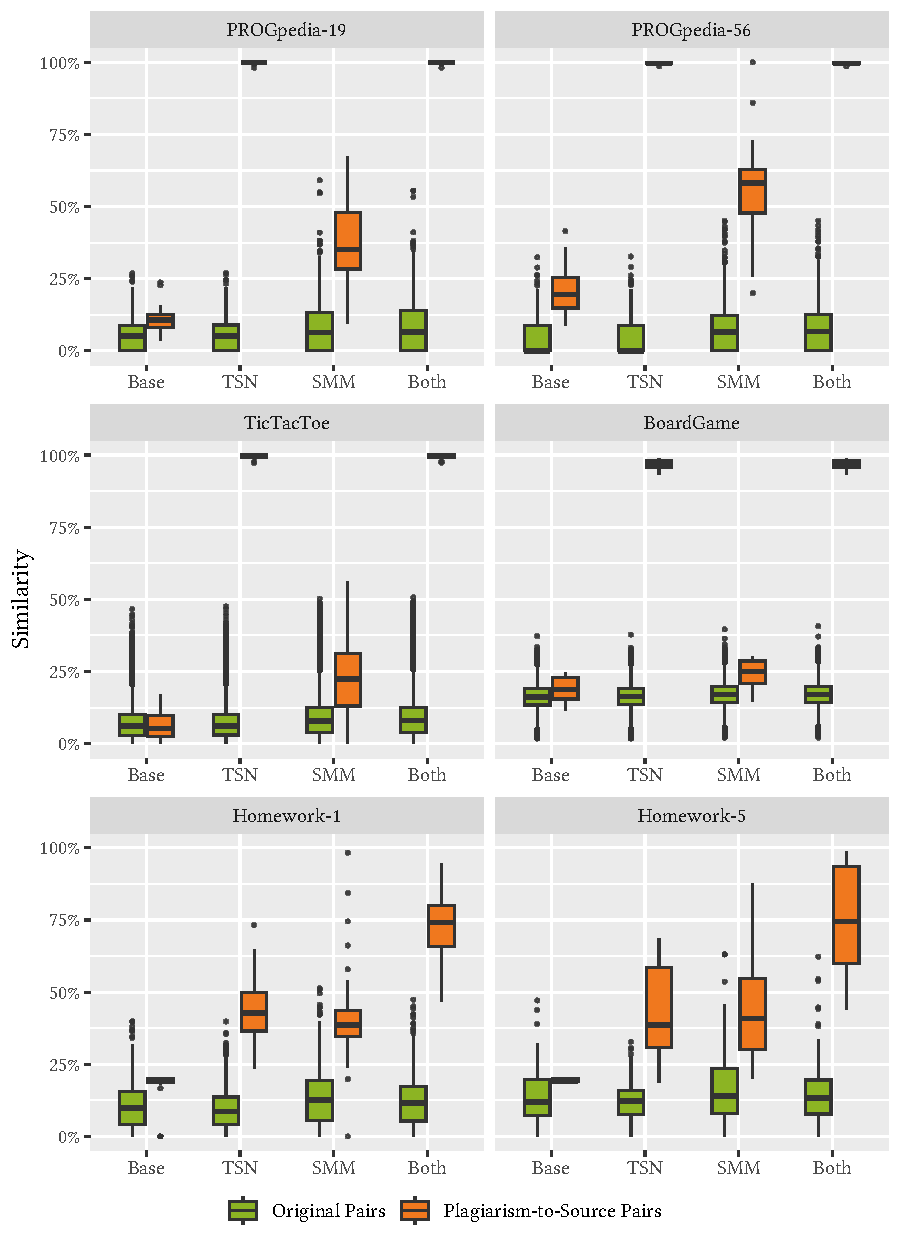
\includegraphics[width=\linewidth]{figures/disseval/eval-insertion_avg.similarity.pdf}
\caption[Evaluation Results: Insertion-based Obfuscation]{Similarity scores for original program pairs and \textbf{insertion-based plagiarism} pairs. Ideally, plagiarism pairs exhibit high similarity, while original pairs should exhibit low similarity.}
\label{fig:stage1-results}
\end{figure}

\subsubsection{Combination of Both}
We see strongly improved results when using both defense mechanisms together compared to the baseline.
With this defense mechanism, we even observe that JPlag is effectively immune to insertion-based attacks.
For the Java dataset, these results mirror the ones for subsequence match merging alone.
For the C++ datasets, however, the combination of both defense mechanisms shows an improvement over each individual.

For all six datasets, \autoref{fig:stage1-results} shows a significant similarity increase for plagiarism pairs (true positives).
Depending on the dataset, the median similarity values rise to between 74.10 percent (Homework-1) and 100.00 percent (PROGpedia-19).
We no longer observe any significant overlap between the plagiarism and original pairs, resulting in a clear separation between both types of pairs.

The median similarity \textit{differences} between plagiarism and original pairs (see \autoref{tab:diff-insert}) now range from 61.22 percentage points (Homework-5) to 93.42  percentage points (PROGpedia-19).
These results show that the combination of both defense mechanisms provides a substantial improvement over the baseline. 

As for both defense mechanisms individually, the improvement when using both is statistically and practically significant (see \autoref{tab:to-base-insert}).
The low p-values indicate statistical significance for the similarity increase for the plagiarism pairs.
Regarding practical significance, the effect size is very large for all of the six datasets.
Our results, thus, show that combining both defense mechanisms provides significant resilience against insertion-based obfuscation attacks for all six datasets.

\summaryBox{1.2}{Our defense mechanisms significantly increase the resilience against semantic preserving insertion-based obfuscation attacks. The median similarity differences increase, depending on the dataset, up to 99.65 percentage points, thus producing a complete separation of plagiarized and original programs. Thus, the degree of resilience effectively reflects near-immunity to insertion-based attacks. As discussed in \autoref{sec:eval-unrel}, the impact on the false positive rate is practically insignificant.}

\subsection{Alteration-based Obfuscation}\label{sec:eval-alter}
% FIGURE TEXT
\autoref{fig:stage2-results} shows the results for obfuscation attacks based on random alterations of the token sequence.
\autoref{tab:diff-alter} shows the corresponding statistical measures.
% ATTACK TYPE REFRESHER TEXT
As discussed, these attacks are simulated, meaning 25\% of the token sequence is directly replaced by another random token. While this is thus not a real obfuscation attack, it simulates the effect of a very strong obfuscation attack. As these simulated alterations could be caused by both semantic-preserving and semantic-altering obfuscation attacks, we consider this evaluation state semantic-agnostic. However, as this simulated obfuscation is done after the tokenization, it cannot be evaluated with the Token Sequence normalization, which partially takes place \textit{during} the tokenization.
Thus, we only evaluate this obfuscation attack for subsequence match merging and the baseline.

\begin{table}[h]
	\centering
	\small
	\begin{tabular}{lrrrrrrrr}
		\toprule
		Dataset                       & Variant & Median    & Mean      & $Q_1$     & $Q_3$     & $\Delta$ Mean & $\Delta$ Median & $\Delta$ IQR \\ 
		\midrule
		\multirow{2}{*}{PROGpedia-19} & Base     & 23.82     & 25.34     & 18.24     & 32.83     & 19.61         & 18.76           & 9.34         \\ 
		                              & SMM      & \B{59.50} & \B{64.33} & \B{55.05} & \B{76.32} & \B{55.17}     & \B{53.15}       & \B{41.85}    \\ 
		\hline
		\multirow{2}{*}{PROGpedia-56} & Base     & 19.92     & 23.16     & 13.90     & 34.22     & 18.27         & 19.92           & 5.13         \\ 
		                              & SMM      & \B{68.59} & \B{66.31} & \B{47.00} & \B{88.70} & \B{58.05}     & \B{62.00}       & \B{34.81}    \\ 
		\hline
		\multirow{2}{*}{TicTacToe}    & Base     & 22.36     & 23.32     & 19.07     & 26.08     & 16.47         & 16.29           & 9.10         \\ 
		                              & SMM      & \B{48.97} & \B{49.48} & \B{42.10} & \B{57.89} & \B{40.65}     & \B{41.13}       & \B{29.58}    \\ 
		\hline
		\multirow{2}{*}{BoardGame}    & Base     & 23.05     & 23.06     & 21.87     & 25.03     & 6.88          & 6.86            & 2.90         \\ 
		                              & SMM      & \B{35.01} & \B{35.06} & \B{33.61} & \B{36.75} & \B{18.11}     & \B{18.05}       & \B{13.87}    \\ 
		\hline
        \multirow{2}{*}{Homework-1}   & Base     & 13.52     & 13.03     & 10.00     & 16.52     & 2.64          & 3.65            & -5.60        \\ 
		                              & SMM      & \B{40.39} & \B{42.23} & \B{33.05} & \B{50.73} & \B{29.19}     & \B{27.81}       & \B{13.55}    \\ 
		\hline
		\multirow{2}{*}{Homework-5}   & Base     & 10.77     & 12.69     & 6.28      & 20.86     & -0.70         & -1.23           & -13.40       \\ 
		                              & SMM      & \B{45.88} & \B{46.32} & \B{37.05} & \B{57.02} & \B{29.95}     & \B{31.86}       & \B{13.37}    \\ 
		\bottomrule
	\end{tabular}
	\caption[Evaluation Results: Alteration-based Obfuscation]{Statistical measures for plagiarism pairs and their differences ($\Delta$) from original pairs for \textbf{alteration-based obfuscation} (corresponds to \autoref{fig:stage2-results}). Higher values indicate better performance. Note that measures are expressed as percentages and their differences as percentage points.}
	\label{tab:diff-alter}
\end{table}

\begin{figure}
\centering
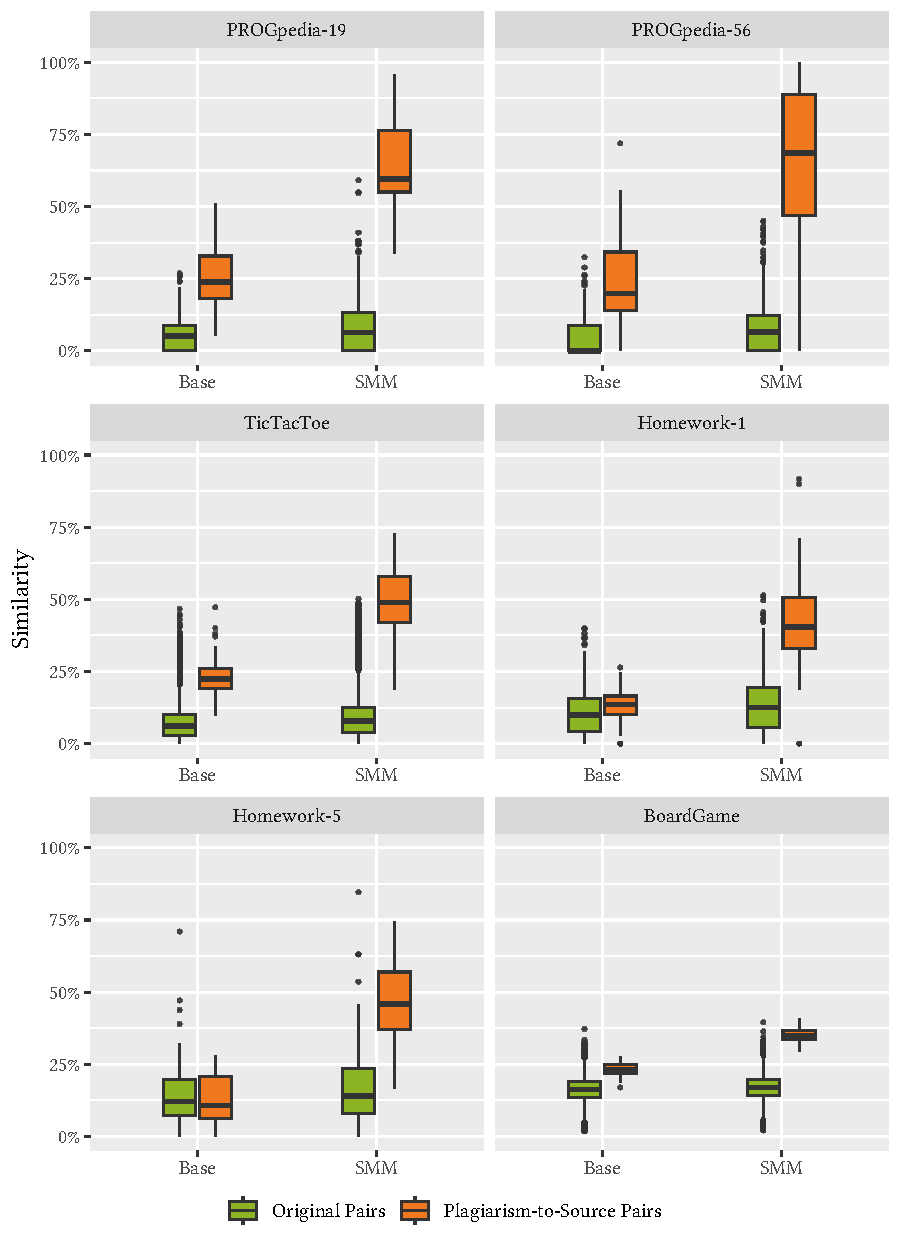
\includegraphics[width=\linewidth]{figures/disseval/eval-alteration_avg.similarity.pdf}
\caption[Evaluation Results: Alteration-based Obfuscation]{Similarity scores for original program pairs and \textbf{alteration-based plagiarism} pairs. Ideally, plagiarism pairs exhibit high similarity, while original pairs should exhibit low similarity.}
\label{fig:stage2-results}
\end{figure}

% ------------------------------------------------------- $
\begin{table}[h]
\centering
\small
%\setlength{\tabcolsep}{5pt}
\begin{tabular}{lrrrrrrrr}
  \toprule
Dataset & Variant & Pairs & $p$ & $W$ & $\delta$ & $\delta\,Int.$ & $\delta$ 95\% CI & n \\ 
  \midrule
   PROGpedia-19& SMM & P2S & 3e-06 & 378 & 0.962 & Very Large & [0.87, 0.99] & 27 \\ 
   PROGpedia-56& SMM & P2S & 3e-06 & 378 & 0.828 & Very Large & [0.59, 0.93] & 28 \\ 
   TicTacToe& SMM & P2S & 3.9e-10 & 1,275 & 0.934 & Very Large & [0.82, 0.98] & 50 \\ 
   BoardGame & SMM & P2S & 4.8e-05 & 210 & 1.000 & Very Large & [1.00, 1.00] & 20 \\ 
   Homework-1& SMM & P2S & < 1e-10 & 1,653 & 0.924 & Very Large & [0.77, 0.98] & 59 \\ 
   Homework-5& SMM & P2S & 0.00011 & 171 & 0.932 & Very Large & [0.75, 0.98] & 18 \\ 
   \bottomrule
\end{tabular}
\caption[Statistical Tests: Alteration-based Obfuscation]{One-sided Wilcoxon signed-rank test results for \textbf{alteration-based obfuscation} regarding the improvement by our defense mechanism compared to baseline (sig. level of $\alpha=0.01$, alternative hypothesis $H1=greater$, test statistic $W$, effect size via Cliff's delta $\delta$, its interpretation $\delta\,Int.$, its 95 percent confidence interval $CI$, and the sample size $n$). For plagiarism-to-source pairs (P2S), low $p$ and high $\delta$ are desirable.} 
\label{tab:to-base-alter}
\end{table}
 
% ------------------------------------------------------- $

\subsubsection{Baseline}
%
\autoref{fig:stage2-results} illustrates the significant impact of the simulated obfuscation attack on the baseline.
For the baseline, the median similarity values for plagiarism pairs (true positives) drop to between 10.77 percent (Homework-5) and 23.82 percent (PROGpedia-19), depending on the dataset.
This results in a clear overlap between plagiarism and original pairs across all datasets.
The overlap is particularly pronounced in the homework datasets, where the interquartile ranges of plagiarism and original pairs strongly intersect.

As shown in \autoref{tab:diff-alter}, the median similarity \textit{differences} between plagiarism and original pairs range from -0.70 percentage points (Homework-5) to 19.61 percentage points (PROGpedia-19). On the lower end, this indicates that the median similarity of plagiarism instances is actually \textit{lower} than that of unrelated programs. Even on the higher end, the difference of 19.61 percentage points offers limited separation between plagiarism pairs and unrelated originals. These baseline results demonstrate that the random alteration simulates the effects of a strong obfuscation attack.

\subsubsection{Subsequence Match Merging}
In contrast to the baseline, subsequence match merging produces strongly improved results.
For all six datasets, \autoref{fig:stage2-results} shows a significant similarity increase for plagiarism pairs (true positives).
The median similarity values rise, depending on the dataset, to between 35.01 percent (BoardGame) and 68.59 percent (PROGpedia-56).
Thus, the overlap is limited and mostly affects the lower quartile of the plagiarism pairs and the upper quartile of the original pairs.
This reduced overlap is also reflected when analyzing the similarity differences between plagiarism and original pairs (see \autoref{tab:diff-alter}).
The median similarity \textit{differences} between plagiarism and original pairs now range from 18.05 percentage points (BoardGame) to 62.00 percentage points (PROGpedia-56).
These results show that subsequence match merging provides a strong improvement over the baseline.

Furthermore, this improvement is clearly both statistically and practically significant, as shown by the results of the statistical test (see \autoref{tab:to-base-alter}).
Regarding statistical significance, the extremely low p-values indicate strong statistical significance for the similarity increase for the plagiarism pairs.
Regarding practical significance, the effect size is very high for all datasets, and thus, the increases are practically significant.
In sum, subsequence match merging provides significant resilience against alteration-based obfuscation attacks for all six datasets.
This means it facilitates detection despite randomly changing 25\% of the linearized program.

\summaryBox{1.3}{Subsequence Match Merging \textit{significantly} increases the resilience against semantic agnostic alteration-based obfuscation attacks. The median similarity differences increase, depending on the dataset, up to 42 percentage points, thus producing a clear separation between plagiarized and original programs. As discussed in \autoref{sec:eval-unrel}, the impact on the false positive rate is practically insignificant.}


\subsection{Refactoring-based Obfuscation}\label{sec:eval-refactor}
% FIGURE TEXT
\autoref{fig:stage2.5-results} shows the results for refactoring attacks based on a mix of different refactoring operations.
\autoref{tab:diff-refactor} shows the corresponding statistical measures.
% ATTACK TYPE REFRESHER TEXT
As discussed, the attack automatically applies semantic-preserving refactoring operations at random positions at the \ac{AST} level to obfuscate programs.
As the implementation of this obfuscation attack~\cite{Maisch2024} only supports Java programs, we evaluate this attack with four of the six datasets.

\begin{table}[h]
	\centering
	\small
	\begin{tabular}{lrrrrrrrr}
		\toprule
		Dataset      & Variant & Median    & Mean      & $Q_1$     & $Q_3$      & $\Delta$ Mean & $\Delta$ Median & $\Delta$ IQR \\ 			
		\midrule
		\multirow{4}{*}{PROGpedia-19} & Base & 18.82     & 23.21     & 14.74     & 29.64      & 17.48         & 13.76           & 5.83         \\ 
		 & TSN  & 18.82     & 22.48     & 14.43     & 27.53      & 16.73         & 13.70           & 5.49         \\ 
		 & SMM  & \B{42.29} & \B{38.63} & \B{27.35} & \B{49.59}  & \B{29.48}     & \B{35.93}       & \B{14.15}    \\ 
		 & Both & 36.26     & 37.15     & 26.23     & 48.21      & 27.93         & 29.69           & 12.35        \\ 
		\hline
		\multirow{4}{*}{PROGpedia-56} & Base & 18.20     & 21.55     & 6.42      & 30.97      & 16.66         & 18.20           & -2.34        \\ 
		 & TSN  & 15.47     & 20.85     & 6.43      & 31.10      & 16.34         & 15.47           & -2.22        \\ 
		 & SMM  & \B{42.62} & 37.02     & 21.33     & \B{50.94}  & 28.76         & \B{36.02}       & 9.13         \\ 
		 & Both & 41.32     & \B{37.21} & \B{24.05} & 50.40      & \B{29.09}     & 34.58           & \B{11.44}    \\ 
		\hline
		\multirow{4}{*}{TicTacToe}    & Base & 13.90     & 17.86     & 9.49      & 22.84      & 11.01         & 7.83            & -0.47        \\ 
		    & TSN  & 13.12     & 17.52     & 8.81      & 22.97      & 10.58         & 6.96            & -1.26        \\ 
		    & SMM  & \B{25.47} & \B{28.84} & \B{16.98} & \B{36.89 } & \B{20.02}     & \B{17.62}      & \B{4.48}     \\ 
		    & Both & 25.28     & 28.00     & 16.91     & 35.93      & 19.08         & 17.32           & 4.28         \\ 
		\hline
		\multirow{4}{*}{BoardGame}    & Base & 35.02     & 35.76     & 29.27     & 39.61      & 19.58         & 18.82           & 10.30        \\ 
		    & TSN  & 34.32     & 35.20     & 28.85     & 39.32      & 18.87         & 17.98           & 9.72         \\ 
		    & SMM  & \B{41.47} & \B{41.37} & \B{35.67} & \B{45.09 } & \B{24.42}     & \B{24.52}       & \B{15.92}    \\ 
		    & Both & 40.40     & 40.54     & 34.16     & 44.16      & 23.45         & 23.32           & 14.26        \\ 
		\bottomrule
	\end{tabular}
	\caption[Evaluation Results: Refactoring-based Obfuscation]{Statistical measures for plagiarism pairs and their differences ($\Delta$) from original pairs for \textbf{refactoring-based obfuscation} (corresponds to \autoref{fig:stage2.5-results}). Higher values indicate better performance. Note that measures are expressed as percentages and their differences as percentage points.}
	\label{tab:diff-refactor}
\end{table}

% ------------------------------------------------------- $
\begin{table}[h]
\centering
\small
\begin{tabular}{lrrrrrrrr}
  \toprule
Dataset & Variant & Pairs & $p$ & $W$ & $\delta$ & $\delta\,Int.$ & $\delta$ 95\% CI & n \\
        \midrule
   \multirow{3}{*}{{PROGpedia-19}}& TSN & P2S & 1 & 11 & -0.036 & Negligible & [-0.33, 0.26] & 27 \\ 
   & SMM & P2S & 6.5e-06 & 325 & 0.567 & Large & [0.28, 0.76] & 27 \\ 
   & Both & P2S & 5e-06 & 350 & 0.510 & Large & [0.21, 0.72] & 27 \\
     \hline
   \multirow{3}{*}{{PROGpedia-56}}& TSN & P2S & 0.31 & 108 & -0.015 & Negligible & [-0.31, 0.28] & 28 \\ 
   & SMM & P2S & 2.2e-05 & 253 & 0.462 & Medium & [0.16, 0.68] & 28 \\ 
   & Both & P2S & 6.5e-06 & 325 & 0.473 & Medium & [0.17, 0.69] & 28 \\ 
   \hline
   \multirow{3}{*}{{TicTacToe}} & TSN & P2S & 0.98 & 143 & -0.020 & Negligible & [-0.24, 0.21] & 50 \\ 
   & SMM & P2S & 5.7e-10 & 1,225 & 0.513 & Large & [0.30, 0.68] & 50 \\ 
   & Both & P2S & 5.7e-10 & 1,225 & 0.484 & Large & [0.27, 0.65] & 50 \\ 
  \hline 
   \multirow{3}{*}{{BoardGame}}& TSN & P2S & 1 & 14 & -0.065 & Negligible & [-0.40, 0.28] & 20 \\ 
   & SMM & P2S & 4.8e-05 & 210 & 0.430 & Medium & [0.06, 0.70] & 20 \\ 
   & Both & P2S & 4.8e-05 & 210 & 0.380 & Medium & [0.01, 0.66] & 20 \\
   \bottomrule
\end{tabular}
\caption[Statistical Tests: Refactoring-based Obfuscation]{One-sided Wilcoxon signed-rank test results for \textbf{refactoring-based obfuscation} regarding the improvement by our defense mechanism compared to baseline (sig. level of $\alpha=0.01$, alternative hypothesis $H1=greater$, test statistic $W$, effect size via Cliff's delta $\delta$, its interpretation $\delta\,Int.$, its 95 percent confidence interval $CI$, and the sample size $n$). For plagiarism-to-source pairs (P2S), low $p$ and high $\delta$ are desirable.} 
\label{tab:to-base-refactor}
\end{table} 
% ------------------------------------------------------- $

\subsubsection{Baseline}
\autoref{fig:stage2.5-results} illustrates the significant impact of refactoring-based obfuscation attack on the baseline.
For the baseline, the median similarity values for plagiarism pairs (true positives) drop to between 13.90 percent (TicTacToe) and 35.02 percent (BoardGame), depending on the dataset.
This results in a clear overlap between plagiarism and original pairs for all datasets except BoardGame. Here, the overlap is less pronounced and mostly affects the outliers of the original pairs. This is in line with the classification proposed in our threat model (see \autoref{fig:clone-types}), which illustrates that more complex obfuscation techniques are harder to apply broadly, which reduces the effectiveness for large programs such as the ones on the BoardGame datasets.

As shown in \autoref{tab:diff-refactor}, the median similarity \textit{differences} between plagiarism and original pairs range from 7.83 percentage points (TicTacToe) to 18.82 percentage points (BoardGame). This indicates a limited separation between plagiarism pairs and unrelated originals. Thus, refactoring is an effective obfuscation on the baseline JPlag.

\subsubsection{Token Sequence Normalization}
As the refactoring-based obfuscation does not rely on statement insertion or reordering, token sequence normalization has little to no effect. This, however, is expected, as it is not designed for refactoring-based obfuscation attacks.

For all six datasets, \autoref{fig:stage2.5-results} shows results that closely resemble the results for the baseline.
The median similarity values of the plagiarism pairs are even a bit lower compared to the baseline for three of four datasets. This reduction, however, is between 0.78 percentage points (TicTacToe) and 2.73 percentage points (PROGpedia-56)). Thus, the reduction is very subtle.
Consequently, this trend is also reflected when analyzing the similarity differences between plagiarism and original pairs (see \autoref{tab:diff-refactor}).
The median similarity \textit{differences} between plagiarism and original pairs range from 6.96 percentage points (TicTacToe) to 18.87 percentage points (BoardGame).

The results of the statistical test (see \autoref{tab:to-base-refactor}), however, show that this change is both statistically and practically insignificant.
Regarding statistical significance, the high p-values indicate no statistical significance similarity increase for the plagiarism pairs.
Regarding practical significance, the effect size even shows a reduction in similarity values through negative values for all three datasets. However, the effect size is close to zero, and the practical significance is thus negligible.
In sum, token sequence normalization provides, as expected, no significant resilience against refactoring-based obfuscation attacks, as the results are not significantly different compared to the baseline.


\subsubsection{Subsequence Match Merging}
In contrast to the baseline, subsequence match merging produces strongly improved results.
For all six datasets, \autoref{fig:stage3-results} shows a significant similarity increase for plagiarism pairs (true positives).
The median similarity values rise, depending on the dataset, to between 25.47 percent (TicTacToe) and 42.62 percent (PROGpedia-56).
Thus, the overlap is limited and mostly affects the lower quartile of the plagiarism pairs and the upper quartile of the original pairs.
This reduced overlap is also reflected when analyzing the similarity differences between plagiarism and original pairs (see \autoref{tab:diff-refactor}).
The median similarity \textit{differences} between plagiarism and original pairs now range from 17.62 percentage points (TicTacToe) to 36.02 percentage points (PROGpedia-56).
These results show that subsequence match merging provides a solid improvement over the baseline. 

Furthermore, this improvement is both statistically and practically significant, as shown by the results of the statistical test (see \autoref{tab:to-base-refactor}).
The low p-values indicate statistical significance for the similarity increase for the plagiarism pairs.
Regarding practical significance, the effect size is medium (BoardGame and PROGpedia-56) to large (TicTacToe, PROGpedia-19) for the datasets, and thus the increases are all practically significant.
In sum, subsequence match merging provides significant resilience against refactoring-based obfuscation attacks for all six datasets.
This means it facilitates detection despite the random application of many refactoring operations, which strongly change the structure of the programs.

\begin{figure}
\centering
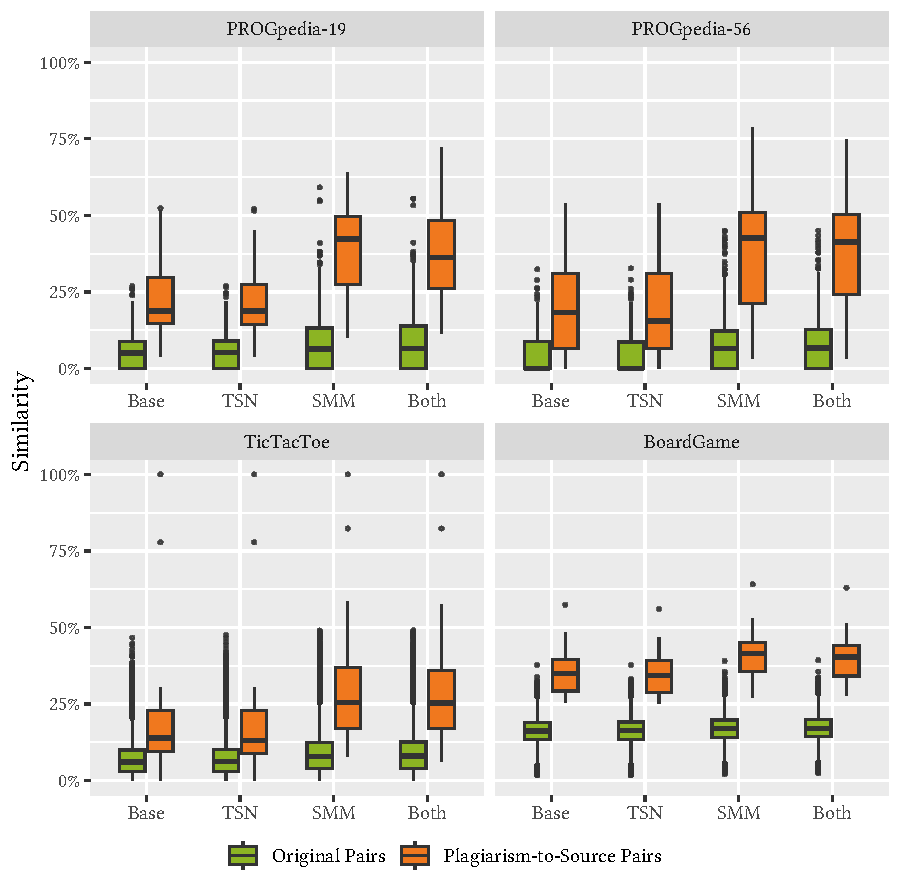
\includegraphics[width=\linewidth]{figures/disseval/eval-refactor_avg.similarity.pdf}
\caption[Evaluation Results: Refactoring-based Obfuscation]{Similarity scores for original program pairs and \textbf{refactoring-based plagiarism} pairs. Ideally, plagiarism pairs exhibit high similarity, while original pairs should exhibit low similarity.}
\label{fig:stage2.5-results}
\end{figure}


\subsubsection{Combination of Both}
When using both defense mechanisms together, we see strongly improved results compared to the baseline.
For all six datasets, \autoref{fig:stage3-results} shows a significant similarity increase for plagiarism pairs (true positives), mirroring the results for subsequence match merging on its own.
Depending on the dataset, the median similarity values rise to between 25.28 percent (TicTacToe) and 41.32 percent (PROGpedia-56).
As for subsequence match merging, the overlap is limited and mostly affects the lower quartile of the plagiarism pairs and the upper quartile of the original pairs.
%This is also reflected when analyzing the similarity differences between plagiarism and original pairs (see \autoref{tab:diff-refactor}).
The median similarity \textit{differences} between plagiarism and original pairs (see \autoref{tab:diff-refactor}) now range from 17.32 percentage points (TicTacToe) to 34.58  percentage points (PROGpedia-56).
Note that these results show a solid improvement over the baseline, which is minimally smaller than the one for subsequence match merging (one exception is PROGpedia-56; here, the combination of both has a slightly higher median difference). 

As for subsequence match merging, this improvement is statistically and practically significant (see \autoref{tab:to-base-refactor}).
The low p-values indicate statistical significance for the similarity increase for the plagiarism pairs.
Regarding practical significance, the effect size is medium (BoardGame and PROGpedia-56) to large (TicTacToe, PROGpedia-19) for the datasets.
In sum, the combination of both defense mechanisms provides significant resilience against refactoring-based obfuscation attacks for all six datasets.

\summaryBox{1.4}{Our defense mechanisms significantly increase the resilience against semantic preserving refactoring-based obfuscation attacks. The median similarity differences increase, depending on the dataset, up to 22 percentage points, thus strongly improving the separation between plagiarized and original programs. As discussed in \autoref{sec:eval-unrel}, the impact on the false positive rate is practically insignificant.}

\subsection{GPT-4-based Obfuscation}\label{sec:eval-gptobf}
% FIGURE TEXT
% ATTACK TYPE REFRESHER TEXT
\autoref{fig:stage3-results} shows the results for obfuscation attacks via GPT-4 prompts. 
\autoref{tab:diff-gpt-obf} shows the corresponding statistical measures.
We used 15 different prompts, asking the LLM to alter the program without changing its behavior. %However, we did not check if the behavior was actually preserved. \todoNils{Wurde das Verhalten manchmal verändert?}
There are no guarantees that the behavior will be preserved, thus making this obfuscation attack a semantic-agnostic one.

It is important to note that the BoardGame dataset was excluded from the evaluation involving AI-based datasets. This dataset originates from a final exam and is highly sensitive. Consequently, we must not submit the programs to the OpenAI server hosting GPT-4 as part of the obfuscation process.

\begin{table}[h]
	\centering
	\small
	\begin{tabular}{lrrrrrrrr}
		\toprule
		Dataset                       & Variant & Median    & Mean      & $Q_1$     & $Q_3$     & $\Delta$ Mean & $\Delta$ Median & $\Delta$ IQR \\ 
		\midrule
		\multirow{4}{*}{PROGpedia-19} & Base     & 54.59     & 54.12     & 28.06     & 81.04     & 48.39         & 49.53           & 19.15        \\ 
		                               & TSN      & 54.74     & 54.84     & 28.82     & 80.95     & 49.08         & 49.61           & 19.88        \\ 
		                               & SMM      & 73.95     & 63.46     & 36.51     & 92.34     & 54.31         & 67.59           & 23.31        \\ 
		                               & Both     & \B{74.79} & \B{63.60} & \B{38.32} & \B{92.98} & \B{54.38}    & \B{68.22}       & \B{24.44}    \\ 
		\hline
		\multirow{4}{*}{PROGpedia-56} & Base     & 66.67     & 61.76     & 46.67     & 77.96     & 56.87         & 66.67           & 37.91        \\ 
		                               & TSN      & 69.40     & 63.92     & 45.05     & 83.92     & 59.40         & 69.40           & 36.41        \\ 
		                               & SMM      & \B{84.43} & \B{75.37} & \B{65.76} & \B{92.60} & \B{67.11}    & \B{77.84}       & \B{53.56}    \\ 
		                               & Both     & 83.07     & 75.10     & 63.11     & 92.59     & 66.98         & 76.32           & 50.50        \\ 
		\hline
		\multirow{4}{*}{TicTacToe}    & Base     & 28.20     & 35.60     & 11.25     & 61.05     & 28.75         & 22.13           & 1.28         \\ 
		                               & TSN      & 27.98     & 37.50     & 12.32     & 62.26     & 30.56         & 21.83           & 2.25         \\ 
		                               & SMM      & \B{39.02} & 44.96     & 17.68     & 75.65     & 36.13         & \B{31.18}       & 5.16         \\ 
		                               & Both     & 38.07     & \B{45.53} & \B{20.11} & \B{75.70} & \B{36.61}     & 30.13           & \B{7.48}     \\ 
		\hline
		\multirow{4}{*}{Homework-1}   & Base     & 19.74     & 27.71     & 9.70      & 42.81     & 17.32         & 9.86            & -5.90        \\ 
		                               & TSN      & 15.47     & 26.44     & 7.88      & 42.50     & 17.07         & 6.83            & \B{-5.77}    \\ 
		                               & SMM      & \B{22.90} & \B{32.69} & \B{10.49} & 48.27     & \B{19.65}     & \B{10.32}       & -9.01        \\ 
		                               & Both     & 19.09     & 31.42     & 8.35      & \B{48.96} & 19.42         & 7.47            & -9.08        \\ 
		\hline
		\multirow{4}{*}{Homework-5}   & Base     & 41.33     & 50.37     & 27.02     & 77.79     & 36.97         & 29.34           & 7.34         \\ 
		                               & TSN      & 36.26     & 46.13     & 20.03     & 73.68     & 34.48         & 23.98           & 4.19         \\ 
		                               & SMM      & \B{50.68} & \B{57.54} & \B{32.45} & 89.24     & \B{41.62}     & \B{36.70}       & \B{8.79}     \\ 
		                               & Both     & 49.06     & 53.90     & 24.40     & \B{90.91} & 39.31         & 35.71           & 4.82         \\ 
		\bottomrule  
	\end{tabular}
	\caption[Evaluation Results: AI-based Obfuscation]{Statistical measures for plagiarism pairs and their differences ($\Delta$) from original pairs for \textbf{AI-based obfuscation} (corresponds to \autoref{fig:stage3-results}). Higher values indicate better performance. Note that measures are expressed as percentages and their differences as percentage points.}
	\label{tab:diff-gpt-obf}
\end{table}


% ------------------------------------------------------- $
\begin{table}[h]
\centering
\small
\begin{tabular}{lrrrrrrrr}
  \toprule
Dataset & Variant & Pairs & $p$ & $W$ & $\delta$ & $\delta\,Int.$ & $\delta$ 95\% CI & n \\ 
  \midrule 
   \multirow{3}{*}{{PROGpedia-19}} & TSN & P2S & 0.0027 & 893 & 0.019 & Negligible & [-0.17, 0.20] & 74 \\ 
   & SMM & P2S & < 1e-10 & 1,485 & 0.210 & Small & [0.02, 0.38] & 74 \\ 
   & Both & P2S & < 1e-10 & 2,216 & 0.209 & Small & [0.02, 0.38] & 74 \\ 
      \hline 
   \multirow{3}{*}{{PROGpedia-56}} & TSN & P2S & 0.025 & 971 & 0.077 & Negligible & [-0.11, 0.26] & 75 \\ 
   & SMM & P2S & < 1e-10 & 1,540 & 0.371 & Medium & [0.19, 0.53] & 75 \\ 
   & Both & P2S & < 1e-10 & 2,136 & 0.360 & Medium & [0.18, 0.52] & 75 \\ 
      \hline
   \multirow{3}{*}{{TicTacToe}} & TSN & P2S & 5.2e-08 & 1,107 & 0.042 & Negligible & [-0.14, 0.22] & 75 \\ 
   & SMM & P2S & < 1e-10 & 1,770 & 0.194 & Small & [0.01, 0.37] & 75 \\ 
   & Both & P2S & < 1e-10 & 2,342 & 0.210 & Small & [0.03, 0.38] & 75 \\ 
      \hline
   \multirow{3}{*}{{Homework-1}} & TSN & P2S & 0.89 & 913 & -0.046 & Negligible & [-0.23, 0.14] & 74 \\ 
   & SMM & P2S & 2e-06 & 406 & 0.075 & Negligible & [-0.11, 0.26] & 74 \\ 
   & Both & P2S & 0.003 & 1,536 & 0.024 & Negligible & [-0.16, 0.21] & 74 \\ 
      \hline
   \multirow{3}{*}{{Homework-5}}& TSN & P2S & 1 & 229 & -0.115 & Negligible & [-0.29, 0.07] & 75 \\ 
   & SMM & P2S & 2.7e-09 & 1,035 & 0.153 & Small & [-0.03, 0.33] & 75 \\ 
   & Both & P2S & 0.11 & 1,260 & 0.047 & Negligible & [-0.14, 0.23] & 75 \\ 
   \bottomrule
\end{tabular}
\caption[Statistical Tests: AI-based Obfuscation]{One-sided Wilcoxon signed-rank test results for \textbf{AI-based obfuscation} regarding the improvement by of our defense mechanism compared to baseline (sig. level of $\alpha=0.01$, alternative hypothesis $H1=greater$, test statistic $W$, effect size via Cliff's delta $\delta$, its interpretation $\delta\,Int.$, its 95 percent confidence interval $CI$, and the sample size $n$). For plagiarism-to-source pairs (P2S), low $p$ and high $\delta$ are desirable.} 
\label{tab:to-base-gpt-obf}
\end{table}
 
% ------------------------------------------------------- $

\subsubsection{Baseline}
\autoref{fig:stage3-results} illustrates the impact of GPT-4-based obfuscation via 15 different prompts.
For JPlag as a baseline, we observe that GPT-based obfuscation attacks can be very effective.
The median similarity values for plagiarism pairs (true positives) drop to between 19.74 percent (Homework-5) and 66.67 percent (PROGpedia-56), depending on the dataset.
Note that this range is higher than usual.

For the different datasets, we observe varying overlaps between plagiarism and original pairs. The strongest overlap is observed for Homework-1, where even the interquartile ranges overlap. The overlap is less pronounced for the PROGpedia datasets.
As shown in \autoref{tab:diff-gpt-obf}, the median similarity \textit{differences} between plagiarism and original pairs range from 9.86 percentage points (Homework-1) to 66.67 percentage points (PROGpedia-56). 
This indicates a limited separation between plagiarism pairs and unrelated originals, especially for the TicTacToe and Homework datasets. 

Note that the variance in the effectiveness of the attack due to the prompt choice is on the same magnitude as the variance between datasets (see \autoref{fig:stage3-results-byprompt}). 
While there are \textit{some} prompts (like prompts 7 and 8) that vary strongly in their effectiveness, most prompts are similar. Interestingly, the dataset itself has arguably a bigger impact on the obfuscation effectiveness than the prompt choice.

It is not surprising that different prompts vary in effectiveness. It is surprising, however, that the effectiveness strongly depends on the dataset. Furthermore, it does not correlate to the language of the datasets, the average size of the programs, or the number of programs in the datasets.
Rather, it seems that it mainly depends on the assignment and the domain to be modeled to solve it.
Consequently, AI-based obfuscation is an effective obfuscation attack. However, it is \textit{less reliable} than algorithmic obfuscation attacks due to the observed high variance.

\begin{figure}
\centering
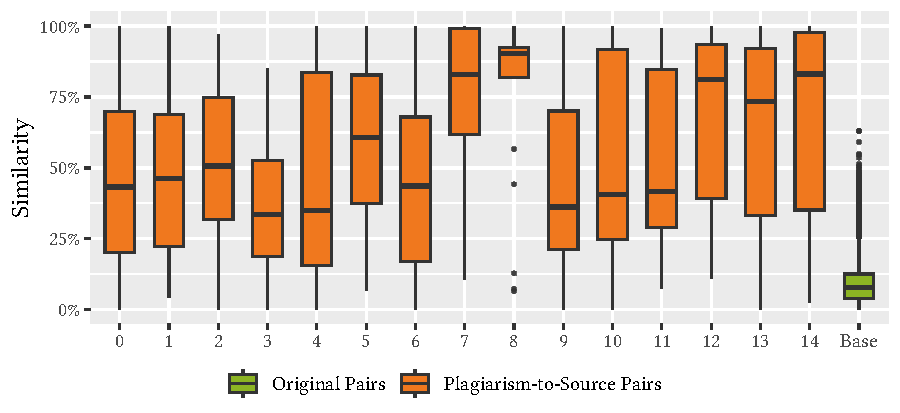
\includegraphics[width=\linewidth]{figures/disseval/eval-chatgpt-obf_avg.similarity-byprompt.pdf}
\caption[Evaluation Results: AI-based Obfuscation by Prompt]{Similarity scores for original program pairs (denoted as \textit{Base}) and \textbf{AI-based plagiarism} pairs by prompt (obfuscation with 15 varying GPT-4 prompts denoted by numbers from 0 to 14). Note that for this illustration, the results of all datasets are merged. Ideally, plagiarism pairs exhibit high similarity, while original pairs should exhibit low similarity.}
\label{fig:stage3-results-byprompt}
\end{figure}


\subsubsection{Token Sequence Normalization}

As GPT-4-based obfuscation relies on various modifications, it is reasonable to expect only a limited effect via token sequence normalization, which targets statement insertion and statement reordering. For all five datasets, \autoref{fig:stage3-results} shows results similar to the baseline.

Depending on the datasets, the median similarity values of the plagiarism pairs (true positives) are either slightly lower or slightly higher compared to the baseline. This difference, however, is minimal, ranging from -5.07 (Homework-5) to 2.37 percentage points (PROGpedia-56). 

We observe a similar effect when looking at the similarity differences between plagiarism and original pairs (see \autoref{tab:diff-gpt-obf}).
The median similarity \textit{differences} between plagiarism and original pairs range from 6.83 percentage points (Homework-1) to 69.40 percentage points (PROGpedia-56).
These values are similar to the baseline. While slightly better for both PROGpedia datasets, they are worse for both Homework datasets, which consist of C++ programs. This could indicate that GPT-4 uses different changes for C++ than for Java code.

The results of the statistical test (see \autoref{tab:to-base-gpt-obf}) show \textit{some} statistical significance; however, they show no practical significance.
Regarding statistical significance, we observe low p-values for the improvements with the PROGpedia-19 and the TicTacToe datasets, thus indicating statistical significance.
For the other three datasets, however, the p-values are above the selected $\alpha$, thus representing statistically insignificant results.
Regarding practical significance, the effect size shows reduced similarity values through negative values for the Homework datasets. However, the effect size is close to zero for all datasets, and the practical significance is thus negligible.
In sum, token sequence normalization provides no significant resilience against GPT-4-based obfuscation attacks. However, it also does not bring any significant drawbacks.


\subsubsection{Subsequence Match Merging}
In contrast to the baseline, subsequence match merging produces strongly improved results.
For all six datasets, \autoref{fig:stage3-results} shows a significant similarity increase for plagiarism pairs (true positives).
Depending on the dataset, the median similarity values rise to between 22.90 percent (Homework-1) and 84.43 percent (PROGpedia-56).
Thus, the overlap is limited and mostly affects the lower quartile of the plagiarism pairs and the upper quartile of the original pairs.
This reduced overlap is also reflected when analyzing the similarity differences between plagiarism and original pairs (see \autoref{tab:diff-gpt-obf}).
The median similarity \textit{differences} between plagiarism and original pairs now range from 10.32 percentage points (Homework-1) to 77.84 percentage points (PROGpedia-56).
These results show that subsequence match merging provides a solid improvement over the baseline. 

Furthermore, this improvement is statistically significant for all datasets and practically significant for all but one, as shown by the results of the statistical test (see \autoref{tab:to-base-gpt-obf}).
Regarding statistical significance, the low p-values indicate strong statistical significance for the similarity increase for the plagiarism pairs.
Regarding practical significance, the effect size varies depending on the dataset. For Homework-1, the effect size is relatively small; thus, the practical significance is negligible (although statistical significance is given).
The effect size for the other five datasets, however, is medium to small, indicating practical significance.
Note that the high variance in plagiarism pair similarities affects the effect size measure~\cite{Grissom2012}. If the data has high variance, it is possible that even with large differences, the overall effect size appears small due to overlapping data points. Due to the use of 15 different prompts, the plagiarism pairs have a high variance in similarity values.

Thus, the increases are practically significant for all but one dataset.
In sum, subsequence match merging provides significant resilience against AI-based obfuscation. As previously stated, the strength of the obfuscation varies strongly on the dataset. Furthermore, the obfuscation attack is semantic agnostic, thus proving a further challenge.
Nevertheless, subsequence match merging improves detection despite AI-based obfuscation leveraging various changes, on which the defense mechanism can make very few assumptions.

\subsubsection{Combination of Both}
When using both defense mechanisms together, we observe strongly improved results compared to the baseline.
For all six datasets, \autoref{fig:stage3-results} shows a significant similarity increase for plagiarism pairs (true positives), mirroring the results for subsequence match merging on its own.
Depending on the dataset, the median similarity values rise to between 19.09 percent (Homework-1) and 83.07 percent (PROGpedia-56).
As for subsequence match merging, the overlap is limited and mostly affects the lower quartile of the plagiarism pairs and the upper quartile of the original pairs.
%This reduced overlap is also reflected when analyzing the similarity differences between plagiarism and original pairs (see \autoref{tab:diff-gpt-obf}).
The median similarity \textit{differences} between plagiarism and original pairs (see \autoref{tab:diff-gpt-obf} now range from 7.47 percentage points (Homework-1) to 76.32 percentage points (PROGpedia-56).
These results show a solid improvement over the baseline, which is minimally smaller than the one for subsequence match merging (one exception is PROGpedia-19; here, it is the other way around). 

This improvement is statistically significant for all datasets but one and practically significant for all but two, as shown by the results of the statistical test (see \autoref{tab:to-base-gpt-obf}).
Regarding statistical significance, the low p-values indicate strong statistical significance for the similarity increase for the plagiarism pairs, with the exception of Homework-5, where the p-value is 0.11.
Regarding practical significance, the effect size varies depending on the dataset. For both homework datasets, the effect size is relatively small; thus, the practical significance is negligible.
It is noteworthy that the homework datasets consist of small C++ programs, where AI-based obfuscation seems more effective. Note that this obfuscation is semantic-agnostic; thus, the behavior of the 75 programs each could deviate from the original.
Nevertheless, the effect size for the other four datasets is medium to small, indicating practical significance. As previously noted, the high variance in plagiarism pair similarities affects the effect size measure, leading to smaller effect size values.

In sum, combining both defense mechanisms provides significant resilience against AI-based obfuscation for the four Java datasets. However, the significance is limited for the two C++ datasets.
Yet, our defense mechanisms improve detection despite the potentially disruptive nature of AI-based obfuscation.

\summaryBox{1.5}{Our defense mechanisms significantly increase the resilience against semantic agnostic AI-based obfuscation attacks. The median similarity differences increase, depending on the dataset, up to 19 percentage points, thus improving the separation between plagiarized and original programs, albeit to a lesser degree than other attack types. As discussed in \autoref{sec:eval-unrel}, the impact on the false positive rate is practically insignificant.}

\begin{figure}
\centering
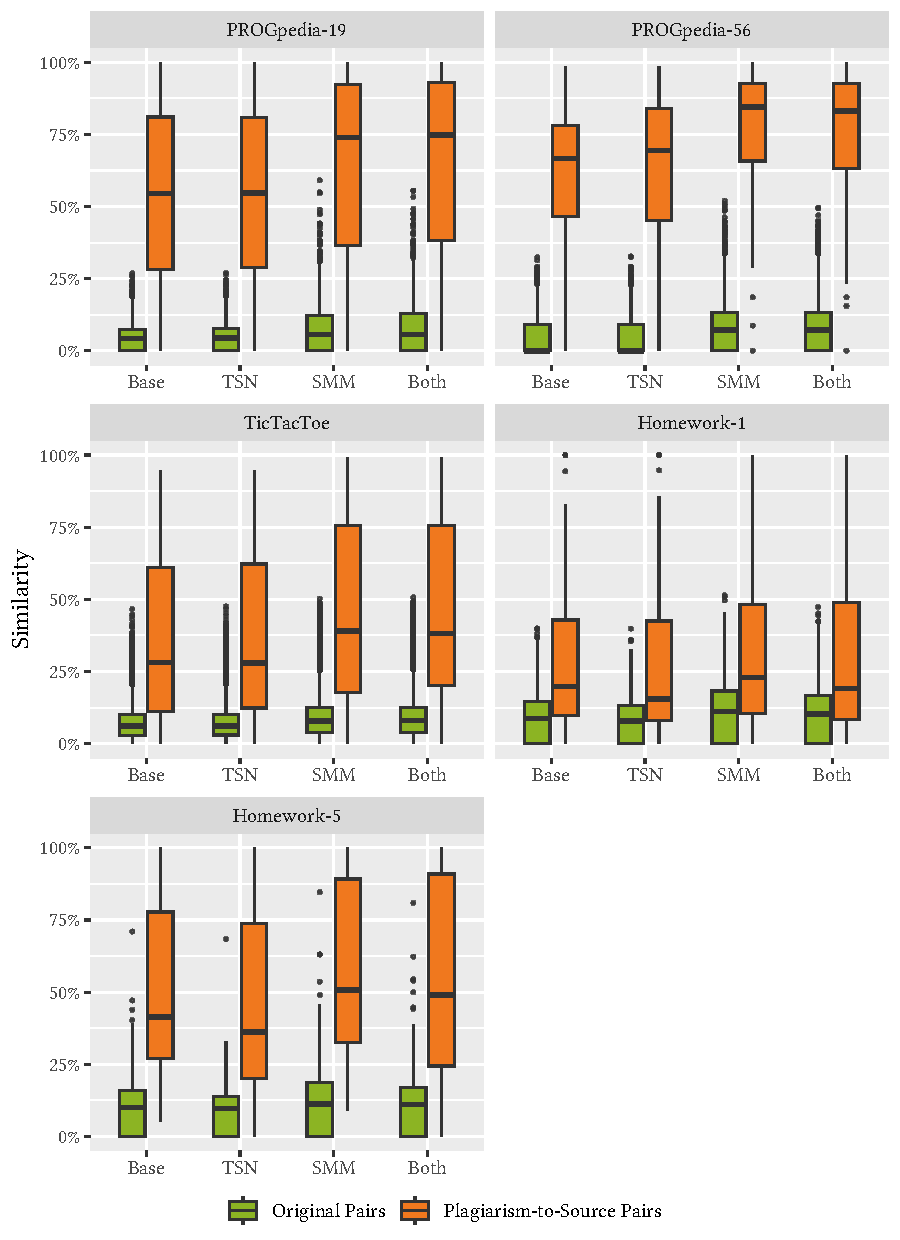
\includegraphics[width=\linewidth]{figures/disseval/eval-chatgpt-obf_avg.similarity.pdf}
\caption[Evaluation Results: AI-based Obfuscation]{Similarity scores for original program pairs and \textbf{AI-based plagiarism} pairs (obfuscation with 15 varying GPT-4 prompts). Ideally, plagiarism pairs exhibit high similarity, while original pairs should exhibit low similarity. }
\label{fig:stage3-results}
\end{figure}

\subsection{GPT-4-generated Programs}\label{sec:eval-gptgen}
\autoref{fig:stage4-results} shows the results for programs generated via GPT-4 based on the assignment description.
\autoref{tab:diff-gpt-gen} shows the corresponding statistical measures.
Unlike in the previous three evaluation stages, we \textit{technically} do not employ obfuscation attacks. The generated programs are not derived from human-made programs. 
Thus, our comparison focuses solely on how the similarity among generated programs differs from that of unrelated human programs.

Although our defense mechanisms are not specifically designed for this scenario, it is worth exploring whether they enhance the detection of AI-generated programs.
If these mechanisms enable us to differentiate between pairs of AI-generated programs and unrelated ones, we can detect AI-generated submissions in practice as long as more than one student chooses to use the same language model.

Since this evaluation stage required the full textual assignment description, we could only perform it on the TicTacToe dataset. As with the previous evaluation stage, the BoardGame dataset and the underlying task were excluded due to their sensitive nature.

\begin{table}[h]
	\centering
	\begin{tabular}{lrrrrrrrrr}
		\toprule
		Dataset                    & Variant & Median    & Mean      & $Q_1$     & $Q_3$     & $\Delta$ Mean & $\Delta$ Median & $\Delta$ IQR \\ 
		\midrule
	    \multirow{4}{*}{TicTacToe} & Base     & 20.63     & 22.53     & 12.53     & 31.51     & 15.67         & 14.57           & 2.57         \\ 
		                           & TSN      & 19.62     & 20.72     & 12.47     & 28.25     & 13.78         & 13.46           & 2.40         \\ 
		                           & SMM      & \B{28.94} & \B{29.60} & \B{18.27} & \B{39.72} & \B{20.77}     & \B{21.10}       & \B{5.75}    \\ 
		                           & Both     & 28.18     & 28.98     & 18.18     & 38.65     & 20.06         & 20.24           & 5.55         \\ 
		\bottomrule
	\end{tabular}
	\caption[Evaluation Results: AI-based Generation]{Statistical measures for plagiarism pairs and their differences ($\Delta$) from original pairs for \textbf{AI-based generation} (corresponds to \autoref{fig:stage4-results}). Higher values indicate better performance. Note that measures are expressed as percentages and their differences as percentage points.}
	\label{tab:diff-gpt-gen}
\end{table}

% ------------------------------------------------------- $
\begin{table}[h]
\centering
\small
%\setlength{\tabcolsep}{5pt}
\begin{tabular}{lrrrrrrrr}
  \toprule
Dataset & Variant & Pairs & $p$ & $W$ & $\delta$ & $\delta\,Int.$ & $\delta$ 95\% CI & n \\ 
  \midrule
   \multirow{3}{*}{{TicTacToe}} & TSN & FG & 1 & 120,687 & -0.072 & Negligible & [-0.12, -0.03] & 1,225 \\ 
    & SMM & FG & < 1e-10 & 334,971 & 0.271 & Small & [0.23, 0.31] & 1,225 \\ 
    & Both & FG & < 1e-10 & 416,672 & 0.256 & Small & [0.21, 0.30] & 1,225 \\ 
   \bottomrule
\end{tabular}
\caption[Statistical Tests: AI-based Generation]{One-sided Wilcoxon signed-rank test results for \textbf{AI-based generation} regarding the improvement by our defense mechanism compared to baseline (sig. level of $\alpha=0.05$, alternative hypothesis $H1=greater$, test statistic $W$, effect size via Cliff's delta $\delta$, its interpretation $\delta\,Int.$, its 95 percent confidence interval $CI$, and the sample size $n$). For Fully-Generated Pairs (FG), low $p$ and high $\delta$ are desirable.} 
\label{tab:to-base-gpt-gen}
\end{table}
 
% ------------------------------------------------------- $

\subsubsection{Baseline}
\autoref{fig:stage4-results} illustrates the results for GPT-4-generated programs.
For the baseline, the similarity values for generated program pairs (true positives) are mostly below 50 percent, with a median similarity of 20.63 percent.
This reflects the inherent indeterminism in generative AI, as these programs were generated from the same assignment description.
However, the similarity of unrelated human-made programs for the same assignment is mostly below 25 percent, with a median similarity of 6.06 percent.
This means that even for our baseline, the generated programs are significantly more similar to each other than human-made programs.

Nevertheless, there is still some overlap. 
As shown in \autoref{tab:diff-gpt-gen}, the median similarity \textit{difference} between AI-generated and original pairs is 14.57 percentage points. 
This indicates a limited separation between human-made and AI-generated programs. Furthermore, this median similarity difference is at a similar level as for refactoring- and alteration-based obfuscation attacks.
However, it is significantly higher than for insertion-based obfuscation attacks, where the median difference was slightly \textit{below} zero (-0.78 percentage points).
In summary, despite the increased similarity of AI-generated programs compared to human-made programs for our baseline, it may still be possible to evade detection, thus motivating the need for mechanisms to improve that.

\subsubsection{Token Sequence Normalization}
As token sequence normalization is designed to deal with statement insertion and statement reordering, we do not expect much impact on AI-generated programs.
AI-generated programs will contain little to no dead code, and the impact of statement order is not big enough on its own.

\autoref{fig:stage4-results} shows, as expected, little to no difference compared to the baseline.
The median similarity of the plagiarism pairs is 19.62 percent, which is slightly lower than the baseline (20.63 percent).
When looking at the similarity \textit{differences} between plagiarism and original pairs (see \autoref{tab:diff-gpt-gen}), we also see a slight reduction, as the difference is 13.46 (instead of 14.57) percentage points when using token sequence normalization.

The results of the statistical test (see \autoref{tab:to-base-gpt-gen}) show that this change is both statistically and practically insignificant.
With a p-value of 1, the improvement when using token sequence normalization over the baseline is not statistically significant.
While the effect size shows a slight reduction in similarity values (thus reflecting the decreased median similarity difference), it is close to zero, and the practical significance is thus negligible.
In sum, token sequence normalization provides, as expected, no significant improvement in resilience against AI-generated programs but also does not have significant drawbacks.

\subsubsection{Subsequence Match Merging}
In contrast to the baseline, subsequence match merging produces strongly improved results.
\autoref{fig:stage4-results} shows a significant similarity increase for plagiarism pairs (true positives).
Compared to the baseline, the median similarity value rises by 8.31 percentage points to 28.94 percent.
Thus, the overlap is decreased and mostly affects the upper quartile of the original pairs.

This reduced overlap is also reflected when analyzing the similarity differences between plagiarism and original pairs (see \autoref{tab:diff-gpt-gen}).
The median similarity \textit{difference} between plagiarism and original pairs is increased to 21.10 percentage points.
These results show that subsequence match merging provides a solid improvement over the baseline.

Furthermore, this improvement is both statistically and practically significant, as shown by the results of the statistical test (see \autoref{tab:to-base-gpt-gen}).
The low p-values indicate strong statistical significance for the similarity increase of the plagiarism pairs.
Regarding practical significance, the effect size is small but still relevant in practice.
In sum, subsequence match merging provides significant improvement for the detection of AI-generated programs.
These results are remarkable, given that the defense mechanism is not designed to detect AI-generated programs. The fact that it improves detection for them is surprising but highlights its versatility.
%This means the defense mechanism facilitates detection despite not being designed to detect AI-generated programs at all.

\subsubsection{Combination of Both}
When using both defense mechanisms together, we observe strongly improved results compared to the baseline.
\autoref{fig:stage4-results} shows a significant similarity increase for plagiarism pairs (true positives), mirroring the results for subsequence match merging.
Compared to the baseline, the median similarity value rises by 7.55 percentage points to 28.18 percent.
As for subsequence match merging, the overlap is decreased and mostly affects the upper quartile of the original pairs.

The median similarity \textit{difference} (see \autoref{tab:diff-gpt-gen}) between plagiarism and original pairs is increased to 20.24 percentage points.
These results show a solid improvement over the baseline, which is insignificantly smaller than the one for subsequence match merging. 

As for subsequence match merging, this improvement is both statistically and practically significant, as shown by the results of the statistical test (see \autoref{tab:to-base-gpt-gen}).
The low p-values indicate strong statistical significance for the similarity increase of the plagiarism pairs, while the effect size suggests practical significance.
In sum, combining both defense mechanisms provides significant improvement in the detection of AI-generated programs.
This improvement is nearly identical to the one for subsequence match merging, so combining both defense mechanisms has no drawbacks.

\summaryBox{1.6}{Our defense mechanisms, while not designed for this purpose, significantly increase the detection rate of AI-generated programs. The median similarity difference to human programs increases by 6.5 percentage points, thus improving the separation between plagiarized and original programs moderately but yet significantly. As discussed in \autoref{sec:eval-unrel}, the impact on the false positive rate is practically insignificant.}


\begin{figure}
\centering
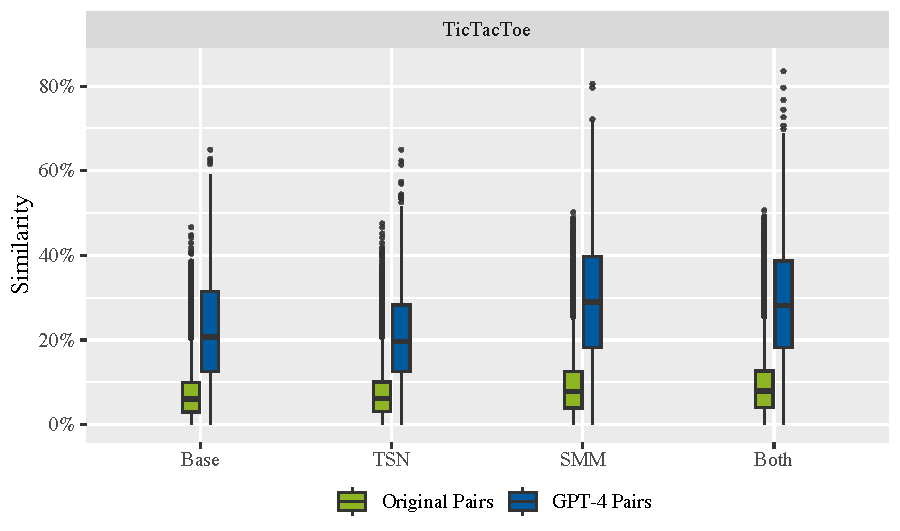
\includegraphics[width=\linewidth]{figures/disseval/eval-chatgpt-full_avg.similarity.pdf}
\caption[Evaluation Results: AI-based Generation]{Similarity scores for original (human) program pairs and pairs of \textbf{AI-generated programs} (based on GPT-4 and the assignment description). Ideally, generated pairs exhibit high similarity, while original pairs should exhibit low similarity.}
\label{fig:stage4-results}
\end{figure}

\subsection{Threshold-based Plagiarism}\label{sec:eval-mossad}

In the previous sections, we evaluated each variant (Base, TSN, SMM, and Both) attack using identical plagiarism instances for a given obfuscation attack.
This allowed us to directly compare the effectiveness of the variants.
Threshold-based obfuscation attacks, like \mossad, rely on a plagiarism detector to verify whether the obfuscated instance is sufficiently dissimilar from its source.
In \autoref{sec:eval-insert}, we configured \mossad to use the baseline (JPlag without defense mechanisms) for this purpose.
This raises the question of how our defense mechanisms affect threshold-based attacks when enabled during the obfuscation process.

To answer this, we chose ten random programs for each of the Homework datasets (\mossad is only compatible with C++ programs) and executed \mossad for each one.
Note that the average size of these programs is small. The Homework-1 dataset has an average size of 105 LoC per program, and the Homework-5 dataset has an average size of 282 LoC per program.
We conducted this evaluation on a system with an AMD Ryzen 7 7700 CPU (8 cores, 16 threads, 3.8 GHz base clock, 5.3 GHz boost), 16 GB of RAM, and Arch Linux (kernel version 6.11.4) as the operating system.
This is a very performant high-end system that could still realistically be used by students.
%
For all programs and variants, \mossad terminated after reaching the target threshold of 25 percent similarity to the original.
However, we observed a notable increase in obfuscation time and inserted statements when using JPlag with our defense mechanisms enabled during the obfuscation.

\autoref{fig:stage5-result-time} presents the results for the obfuscation runtime per program. For the baseline case (JPlag without defense mechanisms), obfuscation takes a median of 24 minutes per program in the Homework-1 dataset and 48 minutes per program in the Homework-5 dataset.
%
With token sequence normalization enabled, the median obfuscation time is increased to 72 minutes per program. Similar times are observed across both datasets despite the larger program sizes in Homework-5.
%
With subsequence match merging enabled, the median obfuscation time rises to 55 minutes for Homework-1 and 110 minutes per program for Homework-5. This indicates a substantial increase in obfuscation time for larger programs in Homework-5. 
%%
When both defense mechanisms are active, median obfuscation time further escalates to 110 minutes per program for Homework-1 and 190 minutes per program for Homework-5. In this configuration, the maximum observed obfuscation times were 234 minutes (nearly four hours) for Homework-1 and 375 minutes (slightly over six hours) for Homework-5.
%
These findings demonstrate that our defense mechanisms enforce a significant computational cost for obfuscation, even on relatively small programs such as those in the Homework datasets. This prolonged obfuscation time poses a notable hurdle to obfuscating plagiarized programs using these methods. However, this alone is not enough to make threshold-based obfuscation ineffective.

\autoref{fig:stage5-result-loc} illustrates the number of inserted statements required to reach the target threshold. Note that we measure the inserted statement relative to the original size of each program to abstract from varying program sizes. One hundred percent thus denotes that the plagiarism instance is double the size of the source program.
%
In the baseline scenario, obfuscation results in a median relative size increase of 87 percent for Homework-1 and 101 percent for Homework-5, nearly doubling the program sizes even without any active defense mechanisms.
%
With token sequence normalization, the required statement insertions rise to a median of 169 percent, nearly tripling the program size across both datasets. As for the obfuscation runtime, the values of both datasets are similar when using token sequence normalization.
%
Using subsequence match merging enabled, the median relative insertion increases to 156 percent for Homework-1 and 169 percent for Homework-5, with obfuscated programs approaching triple their original size.
%%
When both defense mechanisms are active, the median required statement increase reaches 317 percent for Homework-1 and 331 percent for Homework-5, thus quadrupling program size.
The maximum increases we observed were 1193 percent (13 times the original size) for a Homework-1 program and 869 percent (nearly 10 times the original size) for a Homework-5 program.
The lowest observed increases exceeded 200 percent, making every obfuscated program at least three times larger than the original.
%
These results indicate that achieving the obfuscation threshold requires substantial program growth, making obfuscated programs conspicuously large. Such large programs stand out both in manual and tool-based inspection. This means plagiarism detection systems like JPlag can readily flag outliers by considering the number of tokens per program as an additional metric.
%\footnote{Based on the insights from this dissertation, we actually integrated such a metric into JPlag.}.
Consequently, it makes threshold-based obfuscation apparent, thus turning it into an ineffective obfuscation strategy.

%\vspace{-6pt} % ------------------%
In summary, our findings show that obfuscating even small programs requires a significant amount of time, and the resulting plagiarized instances are markedly larger than any other programs in the dataset. Given that our experiments were conducted on a high-performance system with small programs, the time required for obfuscation would be even more prohibitive for larger programs or on less capable systems, potentially extending to days for a single obfuscation attempt. Indeed, obfuscating the 20 programs across all variants took approximately five days (125 hours) in total on our system.
%
Notably, in this evaluation, we set a target similarity threshold of \mossad at 25 percent, while unrelated programs in the dataset typically share a baseline similarity of around 10 to 15 percent. This means to completely avoid any remaining chance of similarity-based detection, an even more aggressive obfuscation with a higher runtime and a higher number of insertions would be required.
This underscores the effectiveness of our defense mechanisms.

%\vspace{-6pt} % ------------------%
Overall, our contributions substantially enhance obfuscation resilience, making threshold-based obfuscation highly time-consuming and resulting in plagiarized solutions that are exceptionally conspicuous due to their size. These factors collectively act as strong deterrents against obfuscation-based plagiarism, making the obfuscation efforts more tedious than completing the actual assignment.
%\vspace{-12pt} % ------------------%

\summaryBox{1.7}{Our defense mechanisms strongly increase the computational cost for threshold-based plagiarism, thus resulting in an obfuscation time of up to 6 hours per program and up to 1300 percent increase in program size, making threshold-based plagiarism more tedious and easily detectable.}

%\summaryBox{1.7}{Our contributions strongly increase the obfuscation duration and the required insertions, making threshold-based obfuscation much more time-consuming and resulting in significantly larger programs that are easily detectable.}

\begin{figure}[p]
\centering
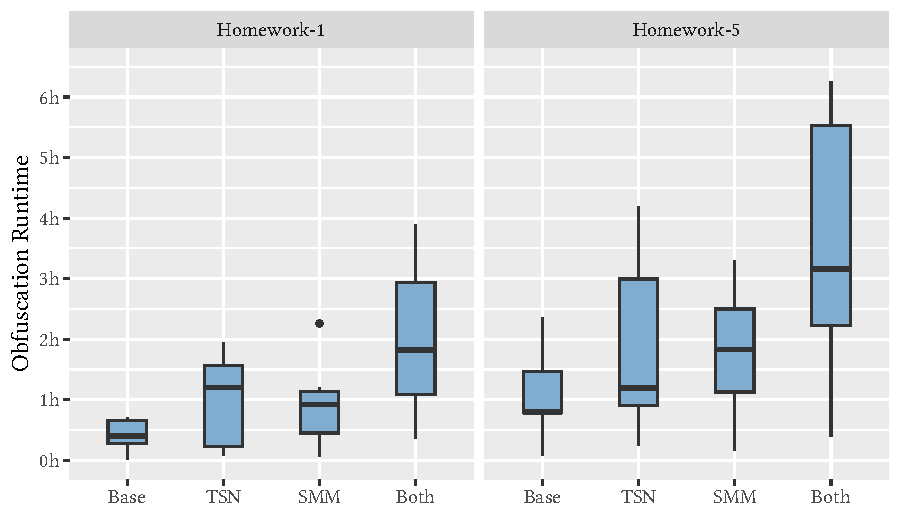
\includegraphics[width=\linewidth]{figures/disseval/eval-MOSSad-runtime_h.pdf}
\caption[Evaluation Results: Obfuscation Duration]{Required obfuscation duration per program for \mossad to reach an obfuscation threshold of 25 percent (for programs with original sizes of \textasciitilde105 LoC for Hw.-1 and \textasciitilde123 LoC for Hw.-5).}
\label{fig:stage5-result-time}
\end{figure}

\begin{figure}[p]
\centering
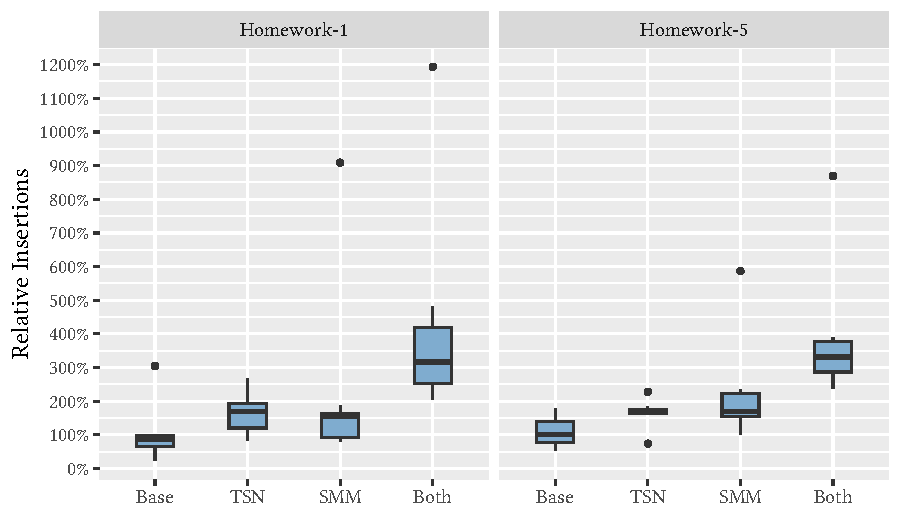
\includegraphics[width=\linewidth]{figures/disseval/eval-MOSSad-insert.pdf}
\caption[Evaluation Results: Inserted Statements]{Required relative insertion of statements for \mossad to reach a 25 percent obfuscation threshold (relative insertions compared to the original program size to normalize for program size).}
\label{fig:stage5-result-loc}
\end{figure}

\section{Result Summary}\label{sec:result-summary}

Our evaluation demonstrates the effectiveness of the proposed defense mechanisms against various obfuscation attack types and their minimal impact on unrelated programs. The results are summarized as follows:

\begin{description}[style=unboxed, leftmargin=0cm]
    \item[Effect on False Positives (\autoref{sec:eval-unrel}):] The defense mechanisms have negligible effects on unrelated programs, ensuring the false-positive rate remains practically insignificant.
    
    \item[Insertion-based Obfuscation (\autoref{sec:eval-insert}):] Token sequence normalization achieves near immunity against insertion-based attacks, with median similarity improvements up to 99.65 percentage points. Subsequence match merging also improves resilience significantly, and combining both mechanisms provides optimal results.
    
    \item[Alteration-based Obfuscation (\autoref{sec:eval-alter}):] Subsequence match merging effectively mitigates alteration-based attacks, achieving median similarity improvements up to 42 percentage points and enabling strong separation of plagiarized and original programs.
    
    \item[Refactoring-based Obfuscation (\autoref{sec:eval-refactor}):] Token sequence normalization minimally impacts refactoring-based attacks, as expected. However, subsequence match merging significantly improves detection, and combining both mechanisms achieves enhanced separation of plagiarized and original programs, with median improvements of up to 22 percentage points.
    
    \item[GPT-4-based Obfuscation (\autoref{sec:eval-gptobf}):] Token sequence normalization has no positive or negative impact on AI-based obfuscation. Subsequence match merging significantly improves resilience against AI-based attacks, with median similarity improvements of up to 19 percentage points. Combining token sequence normalization and subsequence match merging shows similar improvements without drawbacks.
    
    \item[GPT-4-generated Programs (\autoref{sec:eval-gptgen}):] Despite our defense mechanisms not being tailored for AI-generated program detection, we observe improved detection rates. Token sequence normalization has no positive or negative impact on detecting AI-generated programs. Subsequence match merging provides significant improvements, with a median similarity increase of 6.5 percentage points, highlighting its adaptability.
    
    \item[Threshold-based Plagiarism (\autoref{sec:eval-mossad}):] The defense mechanisms substantially increase the computational cost of threshold-based obfuscation, prolonging obfuscation time up to 6 hours per program and inflating program size by up to 1300\%, making such an obfuscation method more tedious and also easily detectable with metrics such as program size or number of tokens.
\end{description}


In summary, our evaluation demonstrates that the proposed defense mechanisms are highly effective across a range of automated obfuscation attacks.
The proposed defense mechanisms provide significantly (statistical and practical significance) improved obfuscation resilience without any practically significant change in false-positive rates.

\section{Discussion}\label{sec:eval-discussion}%\todo{general content: What do the results mean? What can we show? What is our approach good for? Where do its capabilities end?}
In the following, we discuss the interpretation of the evaluation results and highlight key takeaways for software plagiarism detection.
First, we discuss insights regarding the feasibility of the evaluated obfuscation attacks.
Second, we discuss the broad obfuscation resilience our defense mechanisms provide and the relation to our threat model.
Third, we address the issue of outliers and the remaining overlap between plagiarism instances and unrelated programs in detection results and emphasize the importance of human inspection.
Third, we discuss the preservation of program behavior in obfuscation attacks, focusing on the differences between semantic-preserving and semantic-agnostic attacks and how these affect the effectiveness of plagiarism detection.
Next, we analyze the challenges of AI-based plagiarism and explore the effectiveness of AI-based obfuscation and fully generating programs, stressing the need for future re-evaluation.
Finally, we discuss the benefits of layering defense mechanisms, highlighting how integrating multiple approaches enhances obfuscation resilience.

\subsection{Feasibility of Obfuscation Attacks}
Our evaluation results offer key insights into the effectiveness of automated obfuscation techniques against plagiarism detection systems that do \textit{not} include defense mechanisms.

Insertion-based obfuscation is a highly effective strategy, as it significantly hinders the detection of plagiarized programs by adding semantically irrelevant code. Our baseline results show that this method can completely obfuscate plagiarism instances, underscoring the vulnerability of traditional detection systems to this attack type.
%
Refactoring-based obfuscation further exemplifies the challenges posed by obfuscation attacks. Restructuring the program while maintaining its original behavior effectively reduces similarity measures. The baseline results indicate a limited ability to separate plagiarism pairs from unrelated originals, confirming the efficacy of this obfuscation approach.

AI-based obfuscation introduces additional complexity, as AI-based tools are widely available. However, the results reveal significant variability in the effectiveness of these obfuscation attempts, which appears to depend more on the characteristics of the dataset than on prompt design or programming language. While AI-generated obfuscation is powerful, its reliability is lower than that of algorithmic methods, as evidenced by the high variance across datasets. Nevertheless, the semantic-agnostic nature of AI-based obfuscations presents an increasingly relevant challenge to traditional detection systems, emphasizing the need for more sophisticated countermeasures.

AI-generated programs present an emerging challenge. \textit{Currently}, it is only effective for smaller programs. Our results suggest that AI-generated programs exhibit increased similarity to each other compared to human-written programs, which could facilitate detection if multiple students utilize the same model.
The inability to guarantee preserved behavior in AI-generated programs makes them semantic-agnostic.
While not explicitly designed to address this scenario, the findings reveal that subsequence match merging can improve the separation of AI-generated programs from human-written ones.

Threshold-based obfuscation is a unique form of attack that only terminates upon reaching a pre-defined similarity threshold. Although this approach is effective, it inflates the size of programs to obfuscate them, even when targeting detection systems without any defense mechanisms.


\subsection{On Providing Broad Obfuscation Resilience}

The evaluation shows that our approach improves obfuscation resilience for all employed attacks and datasets. As expected, the \textit{degree} of those improvements depends on the type of obfuscation attack. Nevertheless, when employing our defense mechanisms, we demonstrate that the provided resilience is not limited to a specific obfuscation attack. 
We demonstrated effectiveness against various obfuscation attacks, including both algorithmic and AI-based attacks, encompassing semantic-preserving and semantic-agnostic obfuscation.
Furthermore, we evaluate datasets across different programming languages, in addition to diverse assignment types and sizes, thus demonstrating its adaptability.
In total, we use six datasets in combination with five distinct obfuscation attack types. Moreover, each attack type involves various modifications. For example, refactoring-based obfuscation includes multiple transformation types, while AI-based obfuscation involves 15 varying prompts to generate diverse plagiarism instances.

The five obfuscation attack types used in our evaluation align with the different categories outlined in \autoref{fig:clone-types} and discussed in \autoref{sec:threatmodel-categorization}.
For instance, insertion-based obfuscation represents a structural attack, while our alteration-based obfuscation simulates data-based, structural, and complex attacks. Refactoring-based obfuscation falls under the complex attack category. AI-based obfuscation, depending on the specific prompt used, predominantly results in complex attacks. However, some prompts encourage partial replacement of an implementation, placing them in the category of re-implementation. Moreover, detecting AI-generated programs is fundamentally the same problem as detecting re-implementations and, therefore, also falls into this category.

Our contributions enable token-based plagiarism detectors to achieve broad obfuscation resilience across these categories, which was not possible before.
Specifically, as demonstrated by the evaluation results, this includes complete immunity to lexical and data-based attacks, near immunity to structural attacks, strong resilience to complex attacks, and partial resilience to selective re-implementation.

Our evaluation showed that our contributions provide broad resilience against automated obfuscation attacks on programming assignments by systematically covering these different categories of obfuscation attacks. The smallest improvement was observed for AI-based obfuscation, which is expected, given that this is a semantic-agnostic attack using highly challenging prompts, including partial implementations. Detecting partial implementations is particularly difficult for plagiarism detectors as they must carefully balance between detecting re-implementation and avoiding false positives.
On the other hand, the strongest improvement was observed for structural attacks, which is a significant result. Structural attacks are among the easiest to automate, even with traditional methods, and they tend to consistently affect plagiarism detectors. Thus, improving resilience in this area is crucial for the effectiveness of detection tools.


\subsection{Outliers and Remaining Overlap}

Except for insertion-based obfuscation (see \autoref{fig:stage1-results}), where our defense mechanisms completely eliminate \textit{any} overlap between plagiarism instances and unrelated programs, the evaluation results demonstrate minor overlap. This raises an important question regarding the expectations one should have concerning the quality of plagiarism detection.

In practical terms, some overlap among outliers is not a significant concern. It is essential to recognize that no plagiarism detection tool is perfect. Thus, educators must accept that human inspection is always the final step in plagiarism detection and that no one should solely rely on the results of an automated tool without first verifying the flagged candidates themselves. 
%educators must accept that there will always be a possibility of false positives—instances where unrelated programs are mistakenly flagged as suspicious. Nevertheless, these false positives are not common.

Furthermore, it is crucial to note that plagiarism detectors compare pairs of programs, and thus, a single program might be included in multiple comparisons. This means that detecting every plagiarism pair is not necessary to identify all students involved in plagiarism. In practice, educators would be presented with a ranked list of suspicious pairs, which includes both unrelated pairs and plagiarism pairs.

As an example, in our evaluation of GPT-4-generated programs, it is not necessary to identify all 1,225 pairs of AI-generated programs to detect each of the 50 generated programs at least once.
Notably, when both of our defense mechanisms are enabled (\textit{Both} in \autoref{fig:stage4-results}), only the first 158 pairs (which is the top 0.07 percent out of all 220,780 analyzed pairs) need to be inspected to successfully identify 90 percent of the AI-generated programs at least once. To detect all 50 AI-generated programs, the first 711 pairs need to be checked, which is the top 0.3 percent of all pairs, underscoring that a small overlap between the pairs of unrelated programs and the plagiarism pairs is not a cause for concern.

Ultimately, it is important to emphasize that no plagiarism detection tool can provide 100 percent certainty. Therefore, human inspection and informed decision-making are essential in ensuring fair and accurate investigation of misconduct. Educators must \textit{always} engage in thoughtful analysis of the results generated by these tools to effectively discern genuine cases of plagiarism from false positives.

\subsection{Preservation of Program Behavior}

In our evaluation, we employed both semantic-preserving and semantic-agnostic attacks. The former category ensures that program behavior remains intact, while the latter attempts to preserve behavior without providing any guarantees. Notably, AI-based obfuscation attacks, such as those generated by GPT-4, fall into the latter category, where there are no assurances that the program behavior does not change.

For this particular obfuscation attack, we generated a total of 300 plagiarism instances across four datasets, with 75 instances each. Given the scale of our evaluation, it is impractical to verify that these instances did not alter program behavior. While GPT-4 is a sophisticated model, we anticipate that some cases may deviate in behavior. However, this aspect does not undermine our results; instead, it strengthens them. Semantic-agnostic attacks impose fewer constraints, allowing for more substantial changes and a wider variety of alteration types. Consequently, these attacks present a more significant challenge to defend against. Thus, it is noteworthy that our defense mechanisms provide significantly improved resilience for these attacks, even though they are primarily designed to target semantic-preserving attacks.

Under the circumstances of our evaluation, verifying the behavior of the semantic-agnostic plagiarism instances is, therefore, unnecessary. In practical scenarios, students typically strive to maintain the intended behavior of their programs to avoid penalties or lower grades. Therefore, while semantic-altering obfuscation attacks remain an area for future work, the current findings demonstrate the resilience of our defense mechanisms against a variety of obfuscation techniques, including semantic-preserving and semantic-agnostic attacks.


\subsection{AI-based Plagiarism}\label{sec:discussion-ai}
AI-based attacks~\cite{Biderman2022}, particularly those utilizing generative AI, present a growing concern for plagiarism detection.
We discussed two possible scenarios when employing generative AI to cheat on programming assignments. \textit{Automatic obfuscation} of an existing solution and \textit{fully generating} solutions from the assignment description.
%
Based on our evaluation results, automatic obfuscation is \textit{currently} the more effective approach for medium and larger assignments, as fully generating only works well for smaller programs. Generated programs do not fulfill necessary functional requirements (not implementing the required behavior precisely) and even non-functional requirements like code style, thus requiring significant manual effort to improve them sufficiently.
Automatic obfuscation resembles human obfuscation practices, as a pre-existing solution is altered while \textit{trying} to preserve the program behavior.
For both approaches, our defense mechanisms have shown improved resilience.

For AI-generated solutions, there's an ongoing debate on whether this form of cheating\footnote{Obviously, it only constitutes \textit{cheating} if using generative AI is explicitly not allowed in the course.} qualifies as plagiarism~\cite{Novak2019, Saglam2024a}.
Our approach improves the detection rate by helping to recognize the similarities among generated solutions that occur due to the semi-deterministic nature of large language models.
This improvement is surprising, as our defense mechanisms are \textit{not} designed to detect AI-generated programs.

\subsubsection{On the Effectiveness of AI-based Obfuscation}

Our evaluation results show that the effectiveness of our defense mechanisms for AI-based obfuscation is less pronounced compared to their performance against algorithmic attacks. This can be attributed to two key factors.

First, the overall varying effectiveness of AI-based obfuscation plays a significant role. Our results indicate a strong variance in the similarity values achieved by AI-based obfuscation. While part of this variability can be explained by the different prompts used in our evaluation, this trend remains consistent even when examining the results for each prompt individually (see \autoref{fig:stage3-results-byprompt}). For plagiarized programs that already exhibit a high degree of similarity to their original versions, there is limited potential for our defense mechanisms to increase that any further.

Second, generative AI employs a much broader range of modifications compared to algorithmic obfuscation techniques. Algorithmic methods typically rely on a well-defined, limited set of changes during obfuscation. Even refactoring-based obfuscation, which involves multiple refactoring operations, operates within a constrained set of transformations. In contrast, AI-based obfuscation introduces a far more diverse range of modifications, even when using the same prompt. In our evaluation, we observed strong variations in the types of changes applied by AI depending on both the prompt used and the dataset involved. These diverse modifications alter token sequences extensively, posing a challenge to our defense mechanisms.

Nonetheless, it is important to note that our evaluation still shows a notable improvement in resilience against AI-based obfuscation, even in the presence of these complex and varied changes. This demonstrates that while AI obfuscation is an effective technique, our defense mechanisms mitigate its effects.

Interestingly, the effectiveness of AI-based obfuscation attacks strongly varies depending on the dataset used. As illustrated in \autoref{fig:stage3-results}, AI-based obfuscation performs well for Homework-1, while it does not perform well for both PROGpedia datasets. TicTacToe and Homework-5 achieve mixed results. The median similarity differences range, depending on the dataset, between around ten and around 78 percentage points (see \autoref{tab:diff-gpt-obf}).

Although the evaluated plagiarism instances proved to be effective, the process of generating them was not straightforward.
In some cases, GPT-4 produces incomplete or invalid code. Sometimes, the obfuscated programs did not compile, thus requiring re-generation.
%For three original programs, we were not able to produce an acceptable result even after more than 50 attempts.
Despite over 50 attempts, we could not produce a valid result for three original programs, which all exceeded 300 LOC.
%
Thus, algorithmic obfuscation \textit{currently} exhibits more consistent results than AI-based obfuscation, and \textit{currently} can be just as effective.
%However, AI-based obfuscation produces a wide variety of modifications, which could aid in avoiding detection during manual inspection.
However, AI-based obfuscation is more useful in avoiding detection during manual inspection, as it produces diverse modifications and can imitate human-made code.

\subsubsection{On the Effectiveness of AI-based Generation}

While AI-based generation works to a certain extent, its effectiveness is \textit{currently} limited. 
The programs generated entirely by GPT-4 did not fully comply with the specific requirements of the programming assignments, often resulting in additional output or slightly altered behavior.
These discrepancies suggest that fully AI-generated solutions may only be suitable for smaller, less complex assignments.
In our case, the TicTacToe dataset, with a size of approximately 236 lines of code, appears to be near the threshold where fully generated solutions start to exhibit these inconsistencies.

A noteworthy observation is that AI-generated programs are typically shorter than those created by human developers, especially within the TicTacToe dataset. This reduction in length may contribute to the higher degree of similarity observed between AI-generated solutions. While large language models like GPT-4 are not entirely deterministic, they exhibit a level of determinism sufficient for software plagiarism detection purposes. This inherent determinism, coupled with the more concise code produced by AI, may explain why AI-generated programs tend to resemble each other more closely than human-generated ones.

Finally, GPT-4 has a tendency to produce placeholder comments instead of fully implementing certain methods, particularly when the task or method is not well-defined in the prompt. This behavior further limits the effectiveness of AI-based generation for complex assignments, as these incomplete implementations require additional manual intervention to complete.

\subsubsection{Emerging Threats}

While our results thus show that our contributions can effectively address \textit{current} threats of artificial intelligence, rapid advancements in this field may necessitate future re-evaluation. In the future, AI-based obfuscation methods may exhibit less variance in their effectiveness, thus increasing their reliability.
Similarly, new algorithmic attacks might emerge.
%
However, as discussed in our threat model, all emerging attacks must affect the same attack surface (see \autoref{sec:threatmodel-analysis}). Thus, subsequence match merging will provide resilience to emerging attacks. However, the degree of that resilience remains to be assessed.

The rapid development in the field of generative AI may lead to emerging threats that warrant close attention~\cite{Lancaster2023}. One area of particular concern is AI-generated programs. As generative AI advances, this might become feasible for larger programs and produce functionally correct programs for more complex assignments.
%
To detect such fully generated programs, detection systems need capabilities to detect obfuscation via implementation, which can be considered semantic clones. Here, caution is warranted. While matching full re-implementations seems desirable, it risks introducing significant false positives by flagging unrelated programs created independently by students. Note that unrelated solutions to a single problem can also be seen as semantic clones. Thus, we see the danger of creating unreliable detection systems, which may lead to unfairly penalizing students. Addressing re-implementation or semantic clones, therefore, raises philosophical questions about the boundaries of what type of plagiarism we actually want a detection system to target.

For fully generated programs, for example, via generative AI, plagiarism detection methods may not be sufficient for emerging attacks.
If traditional plagiarism detection methods, including the defense mechanisms evaluated in this dissertation, prove inadequate against more sophisticated AI-generated code, alternative techniques may need to be explored~\cite{karnalim2024}. One research area is the development of AI-based detectors that act as countermeasures to generative AI. However, at present, such AI-based detectors have not demonstrated sufficient reliability or performance, and they remain an area of ongoing research~\cite{WeberWulff2023, Pan2024, Khalil_Er_2023}. Another possibility lies in signature- or watermark-based methods, where the artifacts generated by AI are always identifiable as such. This approach would involve recognizing specific patterns or characteristics inherent to AI-generated content, allowing for consistent identification, regardless of the obfuscation techniques applied. Again, this is ongoing research~\cite{zhao2024provable, Jiang2023}. 
%
It is important to note, however, that these potential future developments lie beyond the scope of this dissertation and even outside of the research area of software plagiarism detection.


\subsection{Layering Defense Mechanisms}
Attack-specific defense mechanisms are highly effective, as they can be tailored with strong assumptions about specific obfuscation techniques in mind.
For their targeted obfuscation attacks, attack-specific mechanisms outperform attack-independent approaches.
This is evident in the case of token sequence normalization in \autoref{fig:stage1-results}, where the defense mechanism fully separates plagiarism pairs from original pairs, completely outperforming subsequence match merging.

However, attack-specific mechanisms mostly focus solely on a single known obfuscation attack type. Multiple attack-specific mechanisms must be combined to achieve broad resilience.
Additionally, attack-specific mechanisms can only be designed for known attacks and may not be equipped to handle emerging threats, as they rely on assumptions that may not hold true for unknown obfuscation techniques.

Attack-independent mechanisms, such as subsequence match merging, make fewer assumptions about the obfuscation techniques in use. Thus, they provide less resilience for a given obfuscation attack. 
Their strength, however, lies in providing broad resilience.
Throughout our evaluation, we observed that subsequence match merging consistently offered resilience across a variety of obfuscation attacks.
Because of its heuristic nature and the fact that it operates at a high level of abstraction, it can provide \textit{some} resilience against unknown and emerging obfuscation attacks\footnote{As discussed in \autoref{sec:threatmodel-analysis}, all obfuscation attacks need to affect the token sequence, thus interrupting the subsequence matching, to have any effect on a token-based plagiarism detector.}.
Attack-independent approaches are essential for defending against emerging threats.
Since they make fewer assumptions about the nature of incoming obfuscation attacks, they offer a level of protection against unknown attacks that attack-specific mechanisms may not.

The ideal solution is to combine multiple defense mechanisms, leveraging both attack-specific and attack-independent defense mechanisms.
This strategy provides targeted resilience against well-known or highly effective obfuscation attacks while also offering broad protection against unknown or emerging techniques.
Layering multiple defenses is a well-established strategy in information security and risk assessment, often referred to as the \textit{Swiss cheese model}~\cite{Reason1990} or \textit{defense in depth}~\cite{Stytz2004, Lippmann2006, Anderson2020}.

When using this layered approach, it is critical to ensure compatibility between defense mechanisms to avoid unintended side effects that could reduce overall obfuscation resilience or detection quality.
In the context of software plagiarism detection, it is beneficial to allow users to enable or disable different defense mechanisms depending on their needs or to mitigate potential side effects\footnote{We integrated our defense mechanism into JPlag, allowing educators to benefit from their obfuscation resilience. When using them, it is possible to toggle them as needed for exactly those reasons.}.

Our defense mechanisms are designed to be minimally intrusive, enabling them to be layered with other approaches.
In our evaluation, we examine the combination of defense mechanisms to check for adverse side effects.
While, in some cases, individual mechanisms outperformed combinations, the overall drawbacks of combining them are insignificant.
Therefore, our mechanisms can be safely used in a layered defense strategy.

\section{Threats to Validity}
We now discuss how we address threats to the validity of our evaluation, following the guidelines outlined by \citet{Wohlin2012} and \citet{runeson2008}. These threats apply to the first goal of our evaluation, where we assess obfuscation resilience for programming assignments (\gref{1}). By identifying and mitigating potential threats to internal, external, and construct validity and reliability, we ensure that our findings accurately reflect the effectiveness of our defense mechanisms against automated obfuscation attacks.

\subsection{Internal Validity} 
Internal validity refers to whether there are influences that can unknowingly affect the analyzed variable with respect to causality~\cite{Wohlin2012}.
%

    \textbf{Baseline Consistency:} For internal validity, we used JPlag as a baseline but also implemented our defense mechanism for JPlag, ensuring that all other conditions remained constant when comparing the defense mechanism with each other or with the baseline. 

    \textbf{Handling of invalid programs:} Some public datasets contain invalid or incomplete programs (e.g., programs that do not compile), which could lead to inaccurate results if not properly handled. We addressed this by preprocessing the datasets and removing programs that do not compile. However, even if some cases still remain in the datasets, they do not affect the observed results, as we use the same datasets for the baseline and all of our approaches. 

    \textbf{Validity of the Labeling:} The labels of plagiarism instances in public datasets are often incomplete, incorrect, or solely based on tools like JPlag, which could introduce bias. This threat does not apply in our evaluation, as we use automated obfuscation to generate plagiarism instances (via existing plagiarism generators, obfuscation attack implementation, and large language models). Thus, we have exact labels. As a preprocessing step, we carefully filtered out instances of human plagiarism based on the labels, analyzed them with JPlag, and performed human inspections.

\subsection{External Validity}
External validity concerns the extent to which our findings can be generalized beyond the specific context of the evaluation. % to what extent it is possible to generalize the findings, and to what extent they are of interest to others

    \textbf{Generalizability across datasets:} The datasets used in this evaluation are real-world student submissions from various university courses, thus representing typical scenarios for software plagiarism detection.
    The number and size of programs in the datasets, as well as the choice of programming language, conforms to the typical application of software plagiarism detection, as confirmed by the JPlag developer survey (see \autoref{sec:survey}) and the relevant literature~\cite{Novak2019}.
    We used diverse datasets from different courses, two programming languages, and assignment sizes to improve generalizability and ensure a representative evaluation. This could have been further improved by including a suitable dataset of Python programs, which was not possible due to unavailability. 

    \textbf{Generalizability of obfuscation attacks:}
    Limiting the evaluation to only a few types of obfuscation attacks could hinder the applicability of our results to broader contexts. To enhance external validity and thus ensure that our findings are generalizable, we included a diverse set of obfuscation techniques from all categories outlined in our threat model (see \autoref{sec:threatmodel-categorization}). Note that these are (with the exception of simulated alteration) real-world obfuscation attacks that are, directly or conceptually, available in practice. These steps ensure that our results are relevant to real-world obfuscation threats.

    \textbf{Tool Independence:} Our defense mechanisms are tool-independent, enabling use in token-based and even some other structure-based plagiarism detectors, enhancing their general applicability.
    We evaluated our defense mechanism only using JPlag as the baseline, as other tools are either not applicable to all datasets, closed-source, or provide restricted results. However, this is not a threat to generalizability, as JPlag is considered state-of-the-art~\cite{Novak2019, Aniceto2021} and operates similarly to other widely used tools, reinforcing the generalizability of our findings.

    \textbf{Influence of Prompt Quality:} To address the impact of prompt choice for AI-based obfuscation, we performed systematic "\textit{prompt-engineering}" prior to the evaluation. We then evaluated with 15 different suitable prompts. We generated multiple plagiarism instances for each prompt, which we repeated for multiple datasets. While the impact of the prompt varies (see \autoref{fig:stage3-results-byprompt}), the variation is not strong enough to obscure the overall trend. Thus, we observe consistent patterns of obfuscation resilience across prompts, supporting the generalizability of our results.

\subsection{Construct Validity}
Construct validity refers to how well the evaluation measures its intended purpose and whether the metrics and baselines chosen are appropriate. Thus, it refers to the degree to which we measure theoretical construct we intend to measure.

    \textbf{Evaluation Methodology Alignment:} To enhance construct validity, we aligned our evaluation methodology with those from established and related research works. This ensures that our approach is consistent with the standards in the field. While we deviate from related works by not using a threshold-based classification, we do so specifically to improve internal validity (see \autoref{sec:metrics}), as this method is fundamentally flawed. Finally, we employ an approach-independent ground truth, use established similarity metrics, and a Goal-Question-Metric plan~\cite{Basili1984, Basili1992}.

    \textbf{Underlying Research Object:} We ensure consistency between theoretical research objects and the measurements by maintaining their direct alignment. Since our study evaluates the resilience of software plagiarism detectors against automated obfuscation attacks, we use the similarity scores generated by the detectors as our primary measurement. Additionally, to assess automated obfuscation accurately, we directly utilize real-world plagiarism generators such as \mossad and GPT-4 (which can be exploited to act as one) in our evaluation.
    
    \textbf{Choice of Baseline:} The baseline selection might affect the comparison and outcomes. We addressed this by selecting JPlag as the baseline, as it is widely recognized as a state-of-the-art tool~\cite{Aniceto2021, Novak2019}, ensuring that the comparison is relevant and accurate. As previously mentioned, it operates similarly to other widely used tools by employing standard similarity metrics.

\subsection{Reliability}
Reliability concerns the consistency of the results and whether the study can be replicated under the same conditions.
To ensure reliability, we provide a comprehensive reproduction package for our evaluation~\fancycite{replication-package}.

    \textbf{Use of Internal Datasets:} Using internal datasets can hinder reproducibility. To enhance reliability, we used both public and internal datasets, balancing generalizability with the need for open data where possible. We discussed any preprocessing steps and the employed obfuscation attacks for all datasets.
    For the internal datasets (TicTacToe and BoardGame), we provide raw results and metadata in our replication package. 
    
    \textbf{Consistency across evaluations:} Different datasets vary in size, language, and type of program, which could lead to inconsistent results. We addressed this by using uniform preprocessing steps, evaluation metrics, and statistical tests across all datasets, ensuring that the evaluation was consistent regardless of dataset type or complexity.

    \textbf{Publishing of Obfuscation Attacks:}  The obfuscation attacks utilized in our study can be considered malware, which restricts our ability to provide access to these tools. The exception is GPT-4~\cite{gpt4}, which is publicly available; however, we do not provide a detailed, step-by-step guide on exploiting it for plagiarism detection. While omitting these artifacts or details may hinder reproducibility, balancing this limitation with ethical considerations and the responsibility regarding potential misuse. We aim to ensure that our findings can be reliably assessed while maintaining a commitment to ethical standards.
